\documentclass[11pt,aspectratio=169]{beamer}   % 16:9 slides
\usetheme{Madrid}                              % or any theme you like

\usepackage[utf8]{inputenc}
\usepackage{subcaption}
\usepackage{siunitx}
\sisetup{group-separator={,}}   % 298,939,184.95
\captionsetup{justification=centering,font=small}
\usepackage[T1]{fontenc}
\usepackage{amsmath,amssymb}       % maths in frames
\usepackage{graphicx}              % \includegraphics if you add figures
\usepackage{todonotes}             % provides \todo
\setbeamertemplate{note page}[plain] % nice plain note pages
\setbeameroption{show notes}         % comment out to hide notes


\definecolor{myalert}{RGB}{200,40,40}
\setbeamercolor{alerted text}{fg=myalert}

\title{Optimal Execution with Reinforcement Learning by Team 4}
\author{Team 4}
\date{\today}

\begin{document}
	\begin{frame}[plain]
		\titlepage
	\end{frame}



\begin{frame}{Why Optimal Execution Matters}
	\begin{itemize}
		\item Large orders move prices \textit{(market impact)} – poor execution timing can significantly increase costs.
		\item Execution quality is measured by metrics like Implementation Shortfall (IS) and Expected Shortfall (ES).
		\item Classic solution: \alert{Almgren–Chriss (AC)} model provides an optimal trading schedule under idealized assumptions.
		\item But real markets have richer microstructure: non-linear impact, varying liquidity, fees, etc., challenging the AC model.
	\end{itemize}
\end{frame}

\begin{frame}{The Almgren--Chriss Model}
	\begin{itemize}
		\item Optimal execution cast as a mean–variance trade-off: minimize expected trading cost + $\lambda \times$ (variance of cost).
		\item Assumes simple price dynamics (Arithmetic Brownian Motion with zero drift) and linear market impact.
		\item Temporary impact: each trade incurs a linear price penalty (slippage); Permanent impact: each share traded permanently shifts the price linearly.
		\item Closed-form solution: a static optimal sell schedule parameterized by risk aversion $\lambda$. Varying $\lambda$ traces an efficient frontier of cost vs. risk.
	\end{itemize}
\end{frame}

\begin{frame}{Limitations of the AC Model}
	\begin{itemize}
		\item Assumes price follows a simple arithmetic random walk (no jumps, no changing volatility) or a fixed drift — not true in real markets.
		\item Impact is linear with volume; actual market impact can be non-linear (e.g. higher cost per share for large block trades) and depends on market depth.
		\item Only captures risk via variance of cost; ignores extreme tail-risk and other risk metrics that traders care about.
		\item Yields a static trading schedule – cannot adapt or react to intraday price movement or news once execution begins.
	\end{itemize}
\end{frame}

\begin{frame}{Why Reinforcement Learning?}
	\begin{itemize}
		\item \textbf{Model-free and adaptive:} No need to assume a specific price model – an RL agent can learn the dynamics from data and adjust actions based on real-time price observations.
		\item Naturally handles high-dimensional state inputs (price history, market signals) and continuous action outputs (order sizes).
		\item Can optimize non-linear and custom objectives beyond mean-variance (e.g. directly minimize tail-risk or incorporate transaction costs).
		\item Enables \textbf{dynamic strategies}: policy updates its decisions in reaction to market movements during execution (unlike AC’s static plan).
	\end{itemize}
\end{frame}

% Updated State Representation slide
\begin{frame}{State Representation}
	\textbf{State vector $s_k = [\,r_{k-D+1}, \dots, r_{k},\; m_k,\; i_k\,]$}
	\begin{itemize}
		\item $r_{k-D+1:\,k}$ = window of last $D$ log-returns
		\begin{itemize}
			\item captures recent momentum and volatility in a scale-free manner
			\item $D=5$ is a balance: enough history for trends, but keeps dimensionality low
		\end{itemize}
		\item $m_k = \frac{T-k}{T}$ = fraction of time remaining
		\begin{itemize}
			\item acts as an urgency clock: near end, execution must accelerate regardless of price
		\end{itemize}
		\item $i_k = \frac{Q_k}{Q_0}$ = remaining inventory fraction
		\begin{itemize}
			\item indicates progress: whether most shares remain or execution is nearly complete
		\end{itemize}
	\end{itemize}
	
	\vspace{1em}
	\textbf{Tuning $D$:}
	\begin{itemize}
		\item Shrink ($D\!<5$): faster training, less overfitting, but may miss longer momentum
		\item Expand ($D\!>5$): captures longer autocorrelation, but increases state size and training cost
		\item Treat $D$ as a hyperparameter: grid-search over values (e.g. $\{3,5,8,12\}$) and select via execution-cost vs. risk trade-offs
	\end{itemize}
\end{frame}


\begin{frame}{Action Space}
	\begin{itemize}
		\item Continuous action $a_k \in [0,1]$: the fraction of current remaining inventory to sell at time $k$.
		\item Executed shares $Q_{\text{sell},k} = a_k \times Q_k$ (where $Q_k$ is shares left at step $k$). 
		\item Boundaries: $a_k=0$ means do not trade at this step; $a_k=1$ means sell \textit{all} remaining shares immediately.
		\item This fractional approach naturally prevents overselling and short selling. (Agent cannot sell more than what’s left, and cannot go negative.)
		\item *We will also experiment with alternative action interpretations (e.g. treating $a_k$ as a target trading rate or scaling it by market conditions), but the base case is simple proportional execution.*
	\end{itemize}
\end{frame}

\begin{frame}{Reward Functions in RL Execution}
	\begin{itemize}
		\item \textbf{PnL (Profit and Loss)}: Measures change in portfolio value: $\Delta(\text{Cash} + \text{Inventory} \times \text{Price})$
		\item \textbf{Running Inventory Penalty}: Adds quadratic penalties for holding inventory across time and at terminal step.
		\item \textbf{CjMm Criterion}: PnL $-$ running inventory aversion $-$ terminal inventory mismatch.
		\item \textbf{CjOe Criterion}: PnL $-$ per-step inventory aversion $-$ exponentially weighted leftover impact.
		\item \textbf{Exponential Utility}: $\mathbb{E}[-\exp(-\gamma (X_T + Q_T S_T))]$, introduces strong risk aversion.
		\item \textbf{Normalized Execution Reward}: $(r_t - Q_t P_0) / Q_{\text{total}}$ — normalized version of execution revenue.
		\item \textbf{Execution Shortfall + Penalties}:
		\begin{itemize}
			\item Penalizes shortfall: $Q_t (P_0 - P_t)$
			\item Adds: temporary market impact, leftover penalty, trade smoothness, inventory fraction explosion.
		\end{itemize}
	\end{itemize}
\end{frame}

\begin{frame}{DDPG: Baseline Actor–Critic}
	\begin{itemize}
		\item \textbf{Deep Deterministic Policy Gradient} (Lillicrap \emph{et al.}, 2015)
		\item Off-policy actor–critic for continuous actions
		\item \emph{Actor} $\pi_\phi(s)$ outputs deterministic action $a\in[-1,1]$
		\item \emph{Critic} $Q_\theta(s,a)$ learns value via TD error
		\item Exploration via Ornstein–Uhlenbeck (or Gaussian) noise
		\item \textbf{Pros:} Sample-efficient, reuses replay buffer  
		\item \textbf{Cons:}  
		\begin{itemize}
			\item Over-estimates $Q$ (no double-Q)  
			\item Unstable when reward / dynamics are noisy  
			\item Sensitive to hyperparameters
		\end{itemize}
	\end{itemize}
\end{frame}

\begin{frame}{Deep Deterministic Policy Gradient (DDPG)}
	\begin{itemize}
		\item Off-policy, actor–critic RL algorithm designed for continuous action spaces.
		\item \textbf{Actor:} a neural network $\pi_\theta(s)$ outputs a deterministic action $a$ given state $s$. \textbf{Critic:} a network $Q_\phi(s,a)$ estimates the $Q$-value (expected return) of state-action pairs.
		\item Learns via alternating updates: Critic learns by minimizing TD error; Actor learns by gradient ascent on $Q$ (improve actions w.r.t. critic’s evaluation).
		\item Uses experience replay (random mini-batches from past experiences) and target networks for stability. Exploration is driven by adding noise (e.g. Ornstein–Uhlenbeck process) to the actor’s actions during training.
	\end{itemize}
\end{frame}

\begin{frame}{Dense vs. Sparse Rewards}
	\begin{itemize}
		\item \textbf{Dense:} Agent receives reward feedback at each time step (e.g. based on the immediate trading cost or P\&L change after each action).
		\item \textbf{Sparse:} Agent receives zero reward during the episode and only gets a final reward at the end (based on total execution cost or utility).
	\end{itemize}
	\pause
	\textit{Observation:} Dense rewards tended to accelerate learning (more frequent feedback), whereas sparse rewards encouraged more risk-aware behavior but required longer training to converge.
	\vspace{0.5em}
\end{frame}

\begin{frame}{Sparse Rewards}
	\begin{figure}[ht]
		\centering
		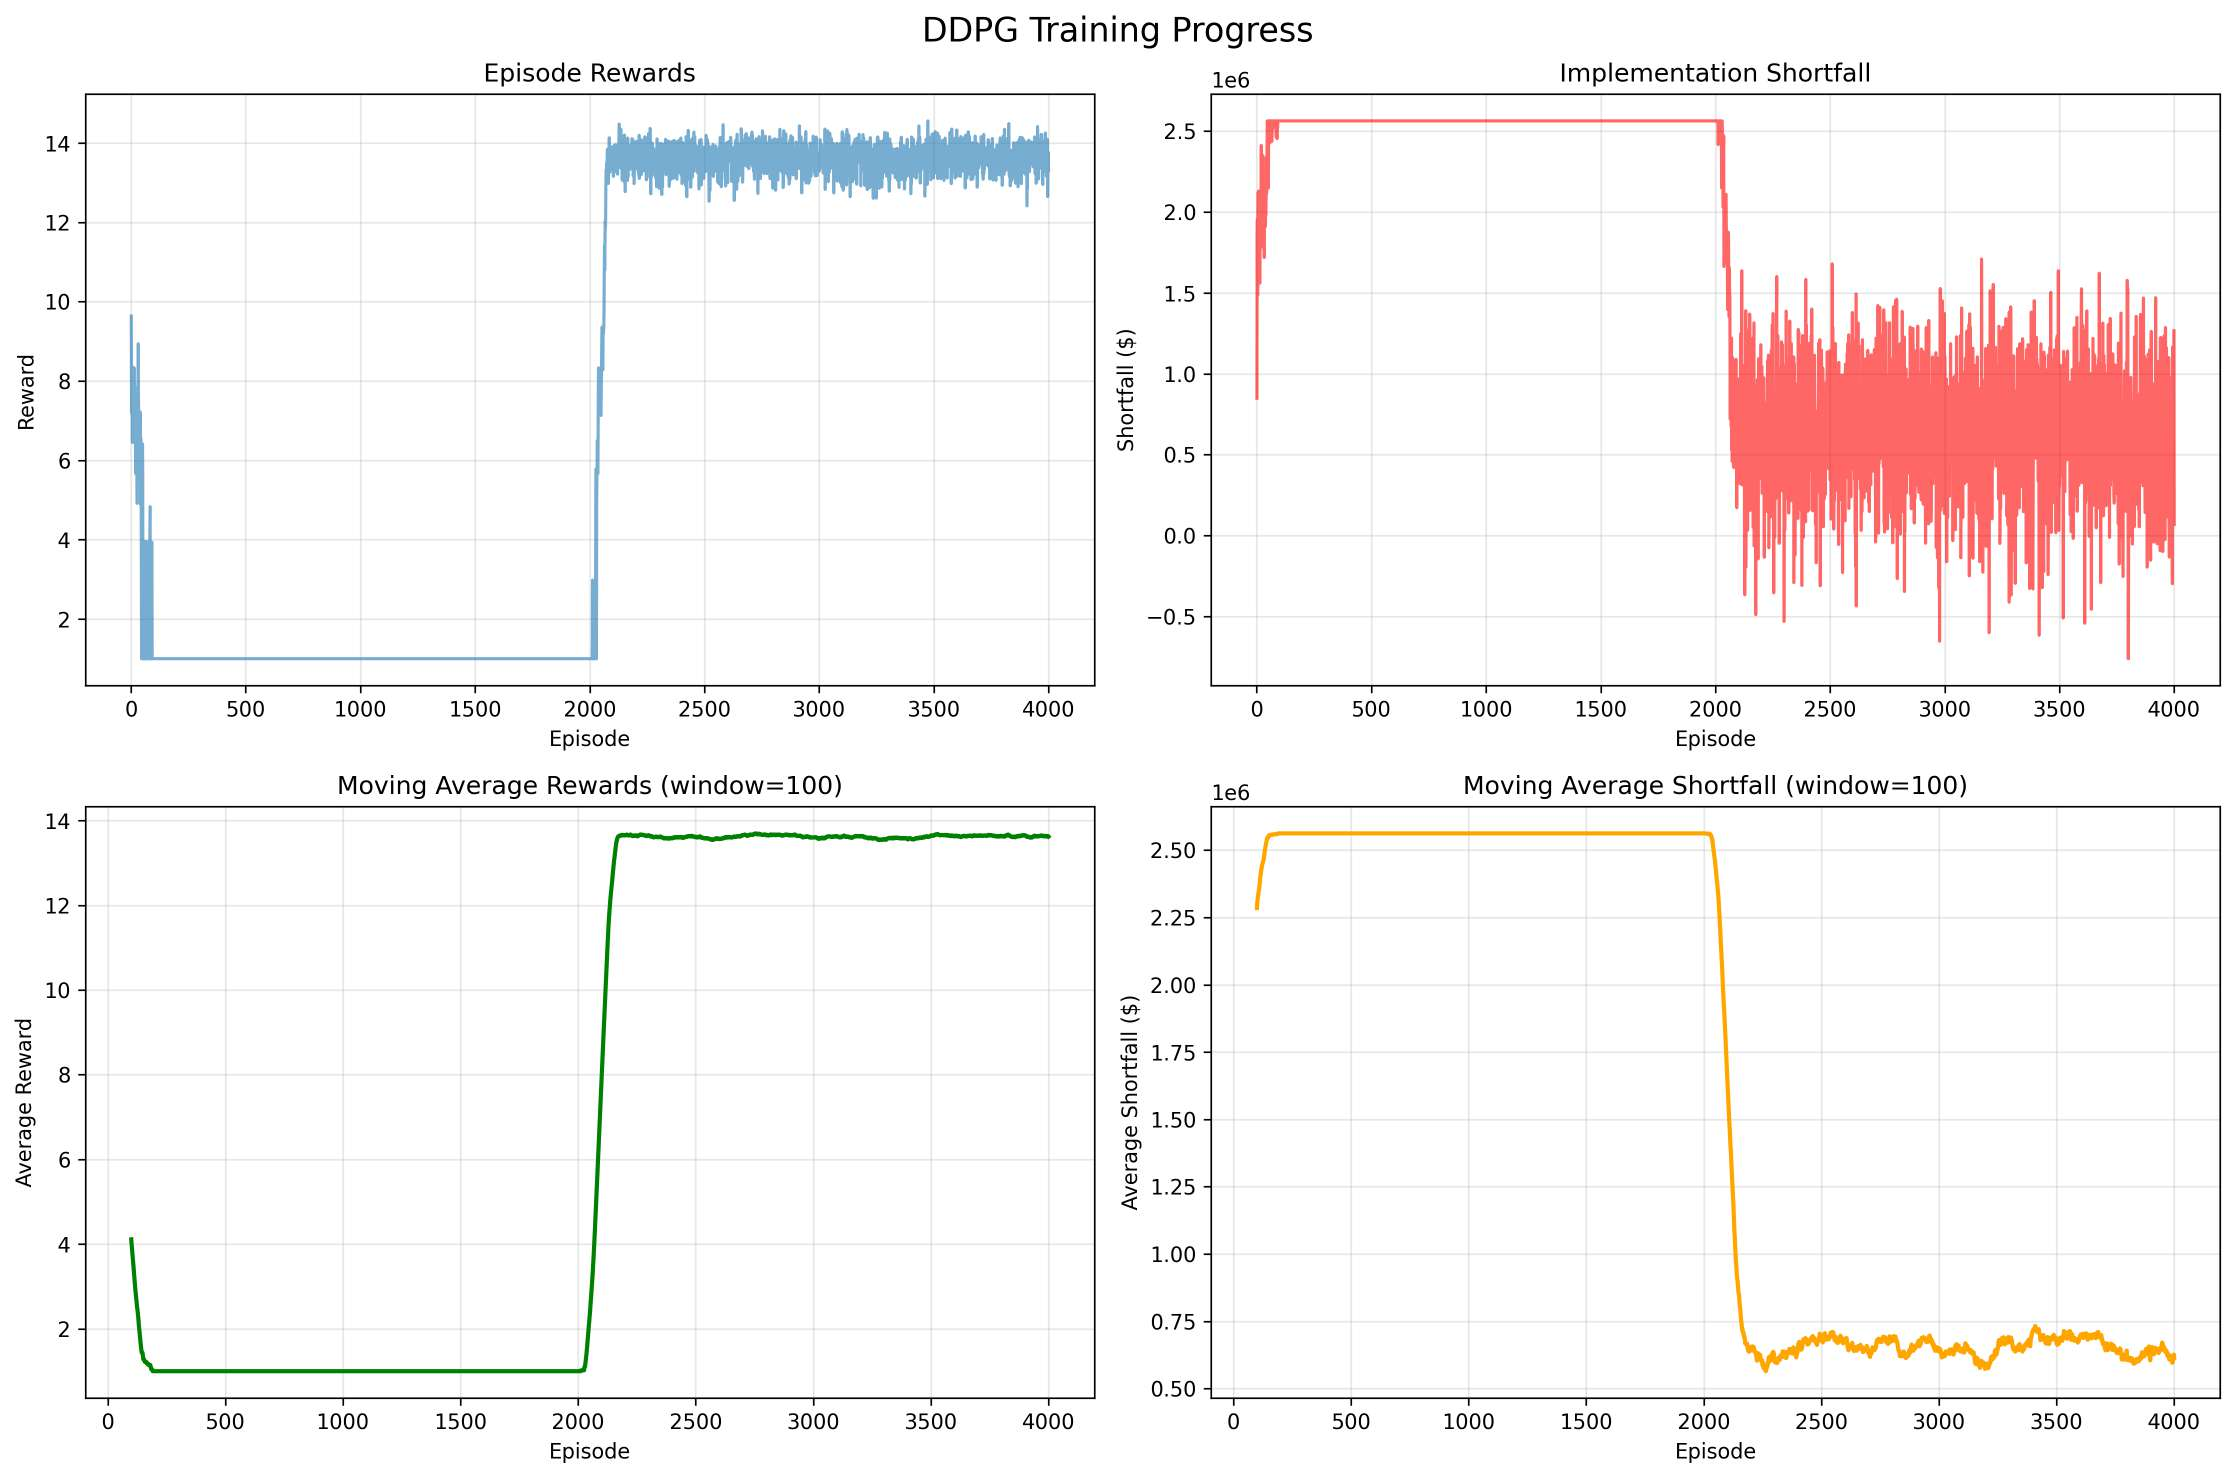
\includegraphics[width=0.6\linewidth]{training_progress.pdf}
		\caption{ddpg baseline training progress}
	\end{figure}
\end{frame}

\begin{frame}{Sparse Rewards}
	\begin{figure}[ht]
		\centering
		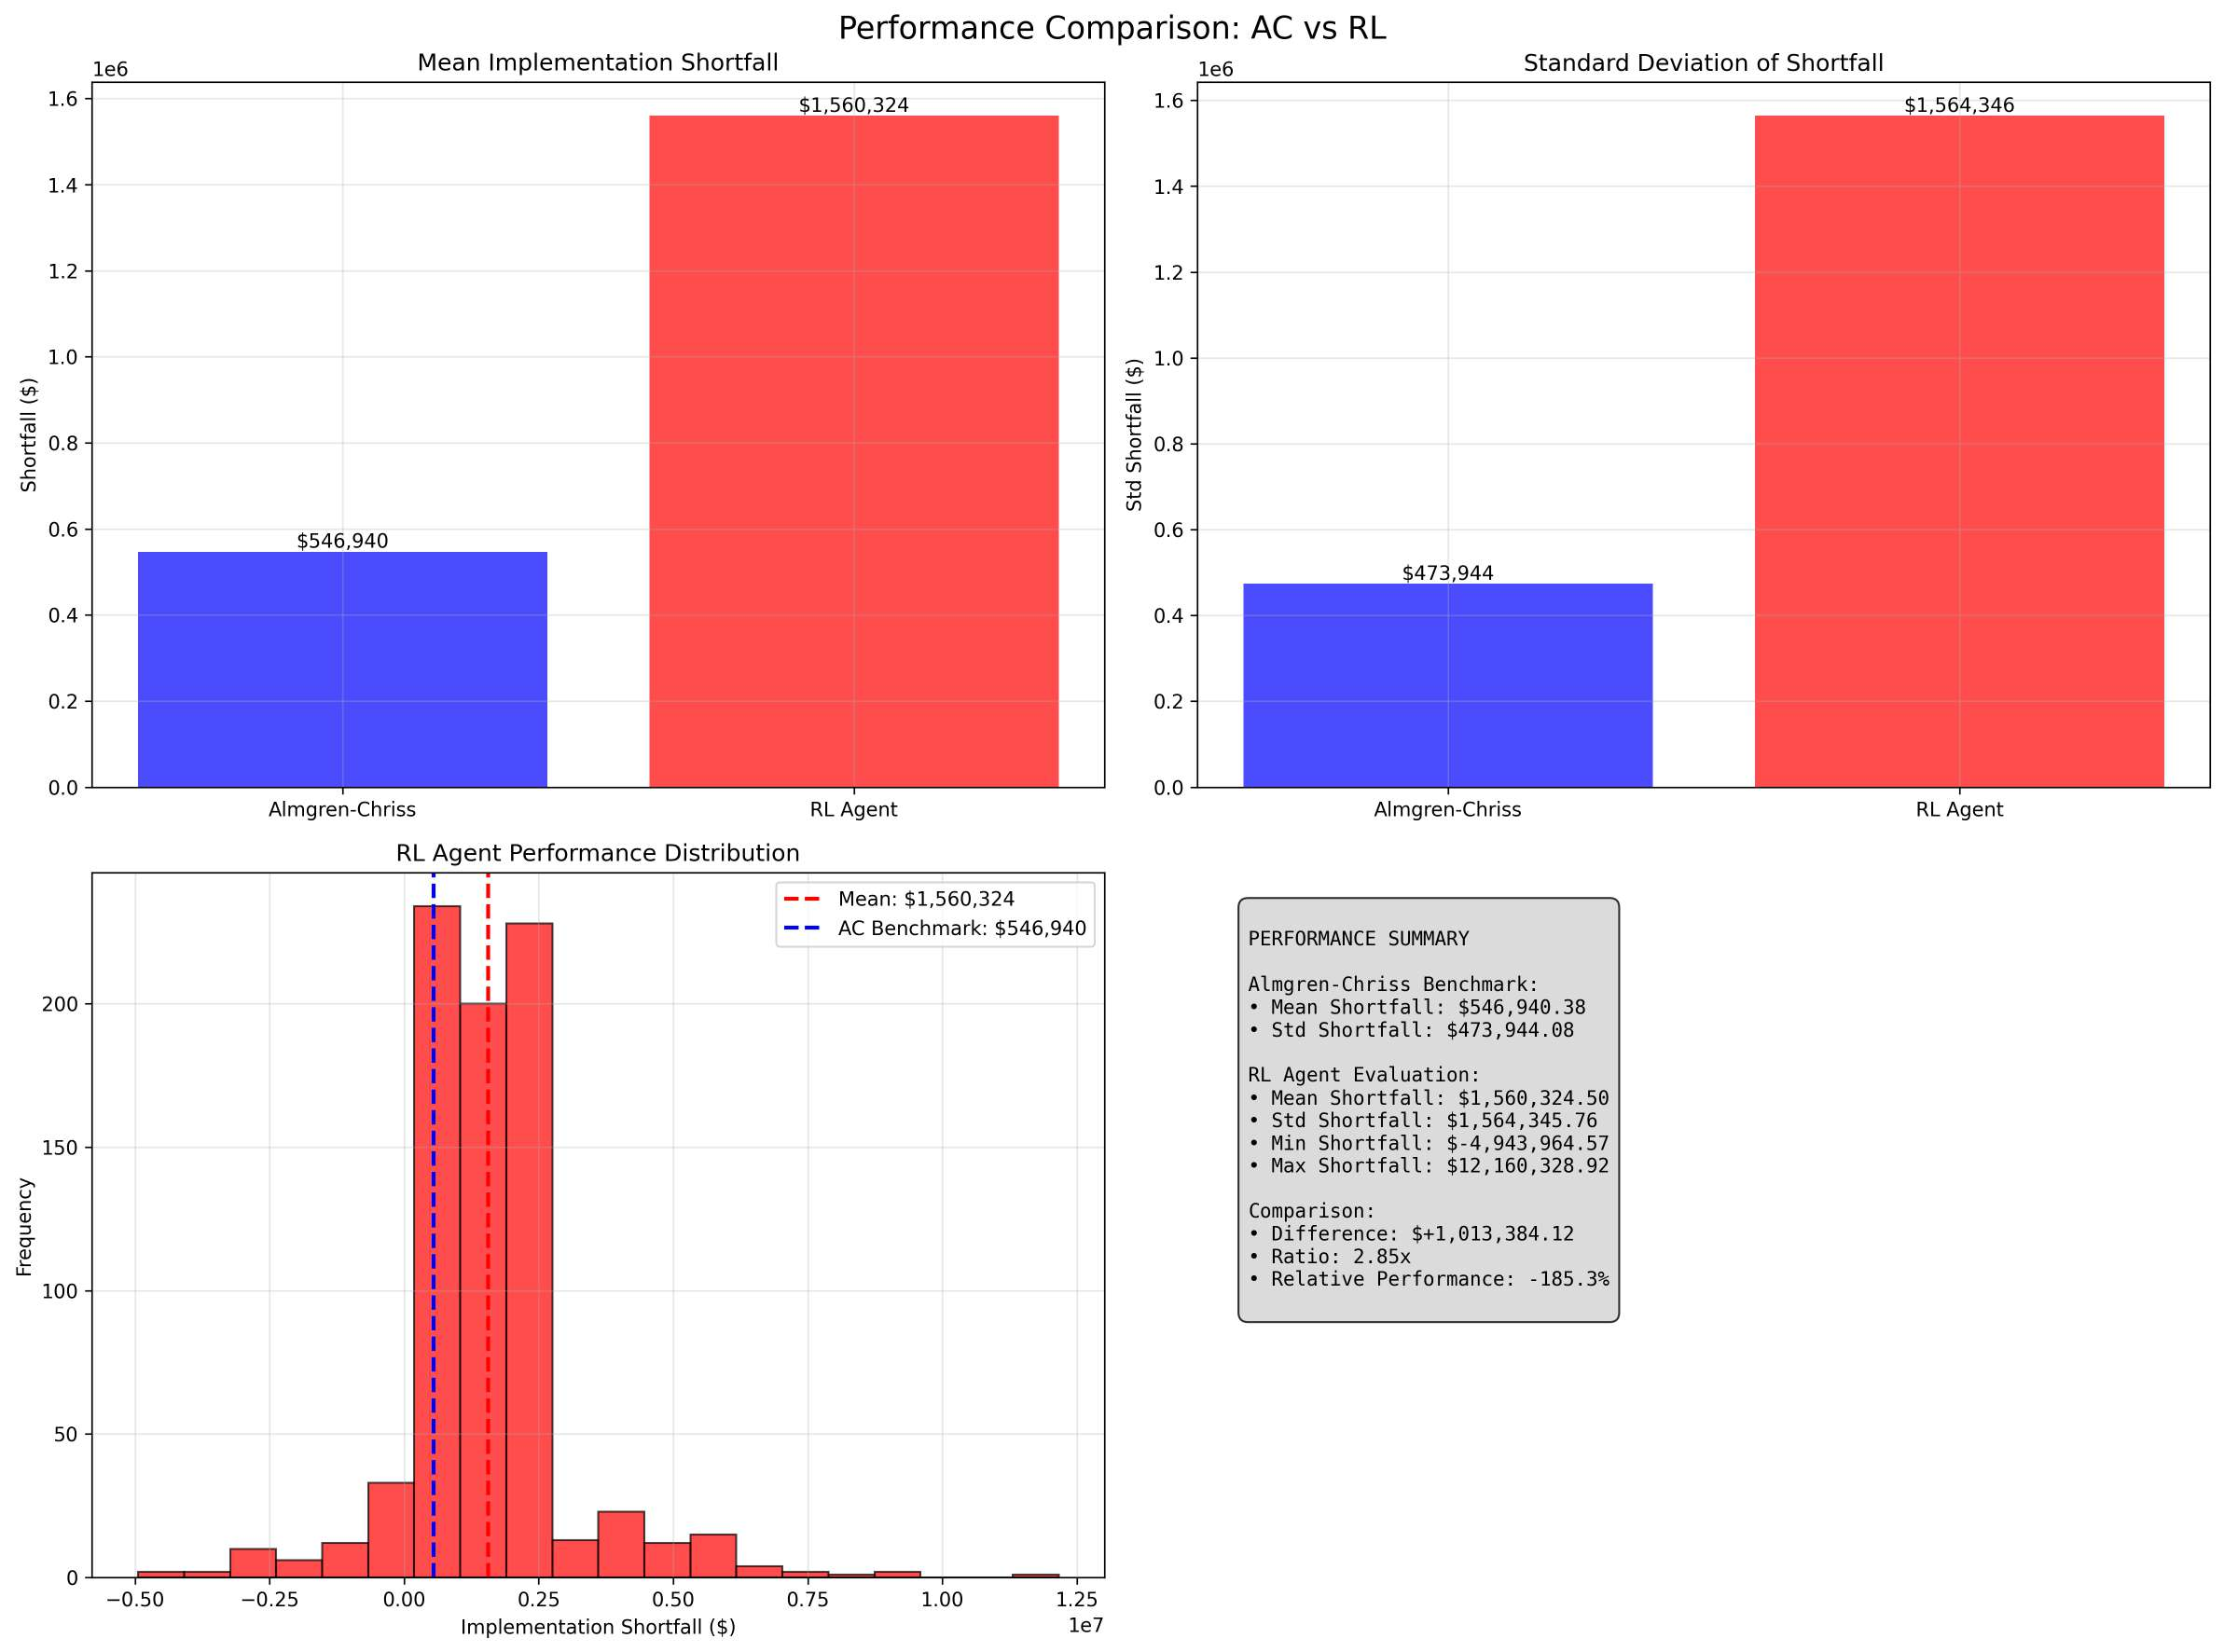
\includegraphics[width=0.6\linewidth]{performance_comparison_baseline.pdf}
		\caption{comparison with the given model}
	\end{figure}
\end{frame}

\begin{frame}{Sparse Rewards}
	\begin{figure}[ht]
		\centering
		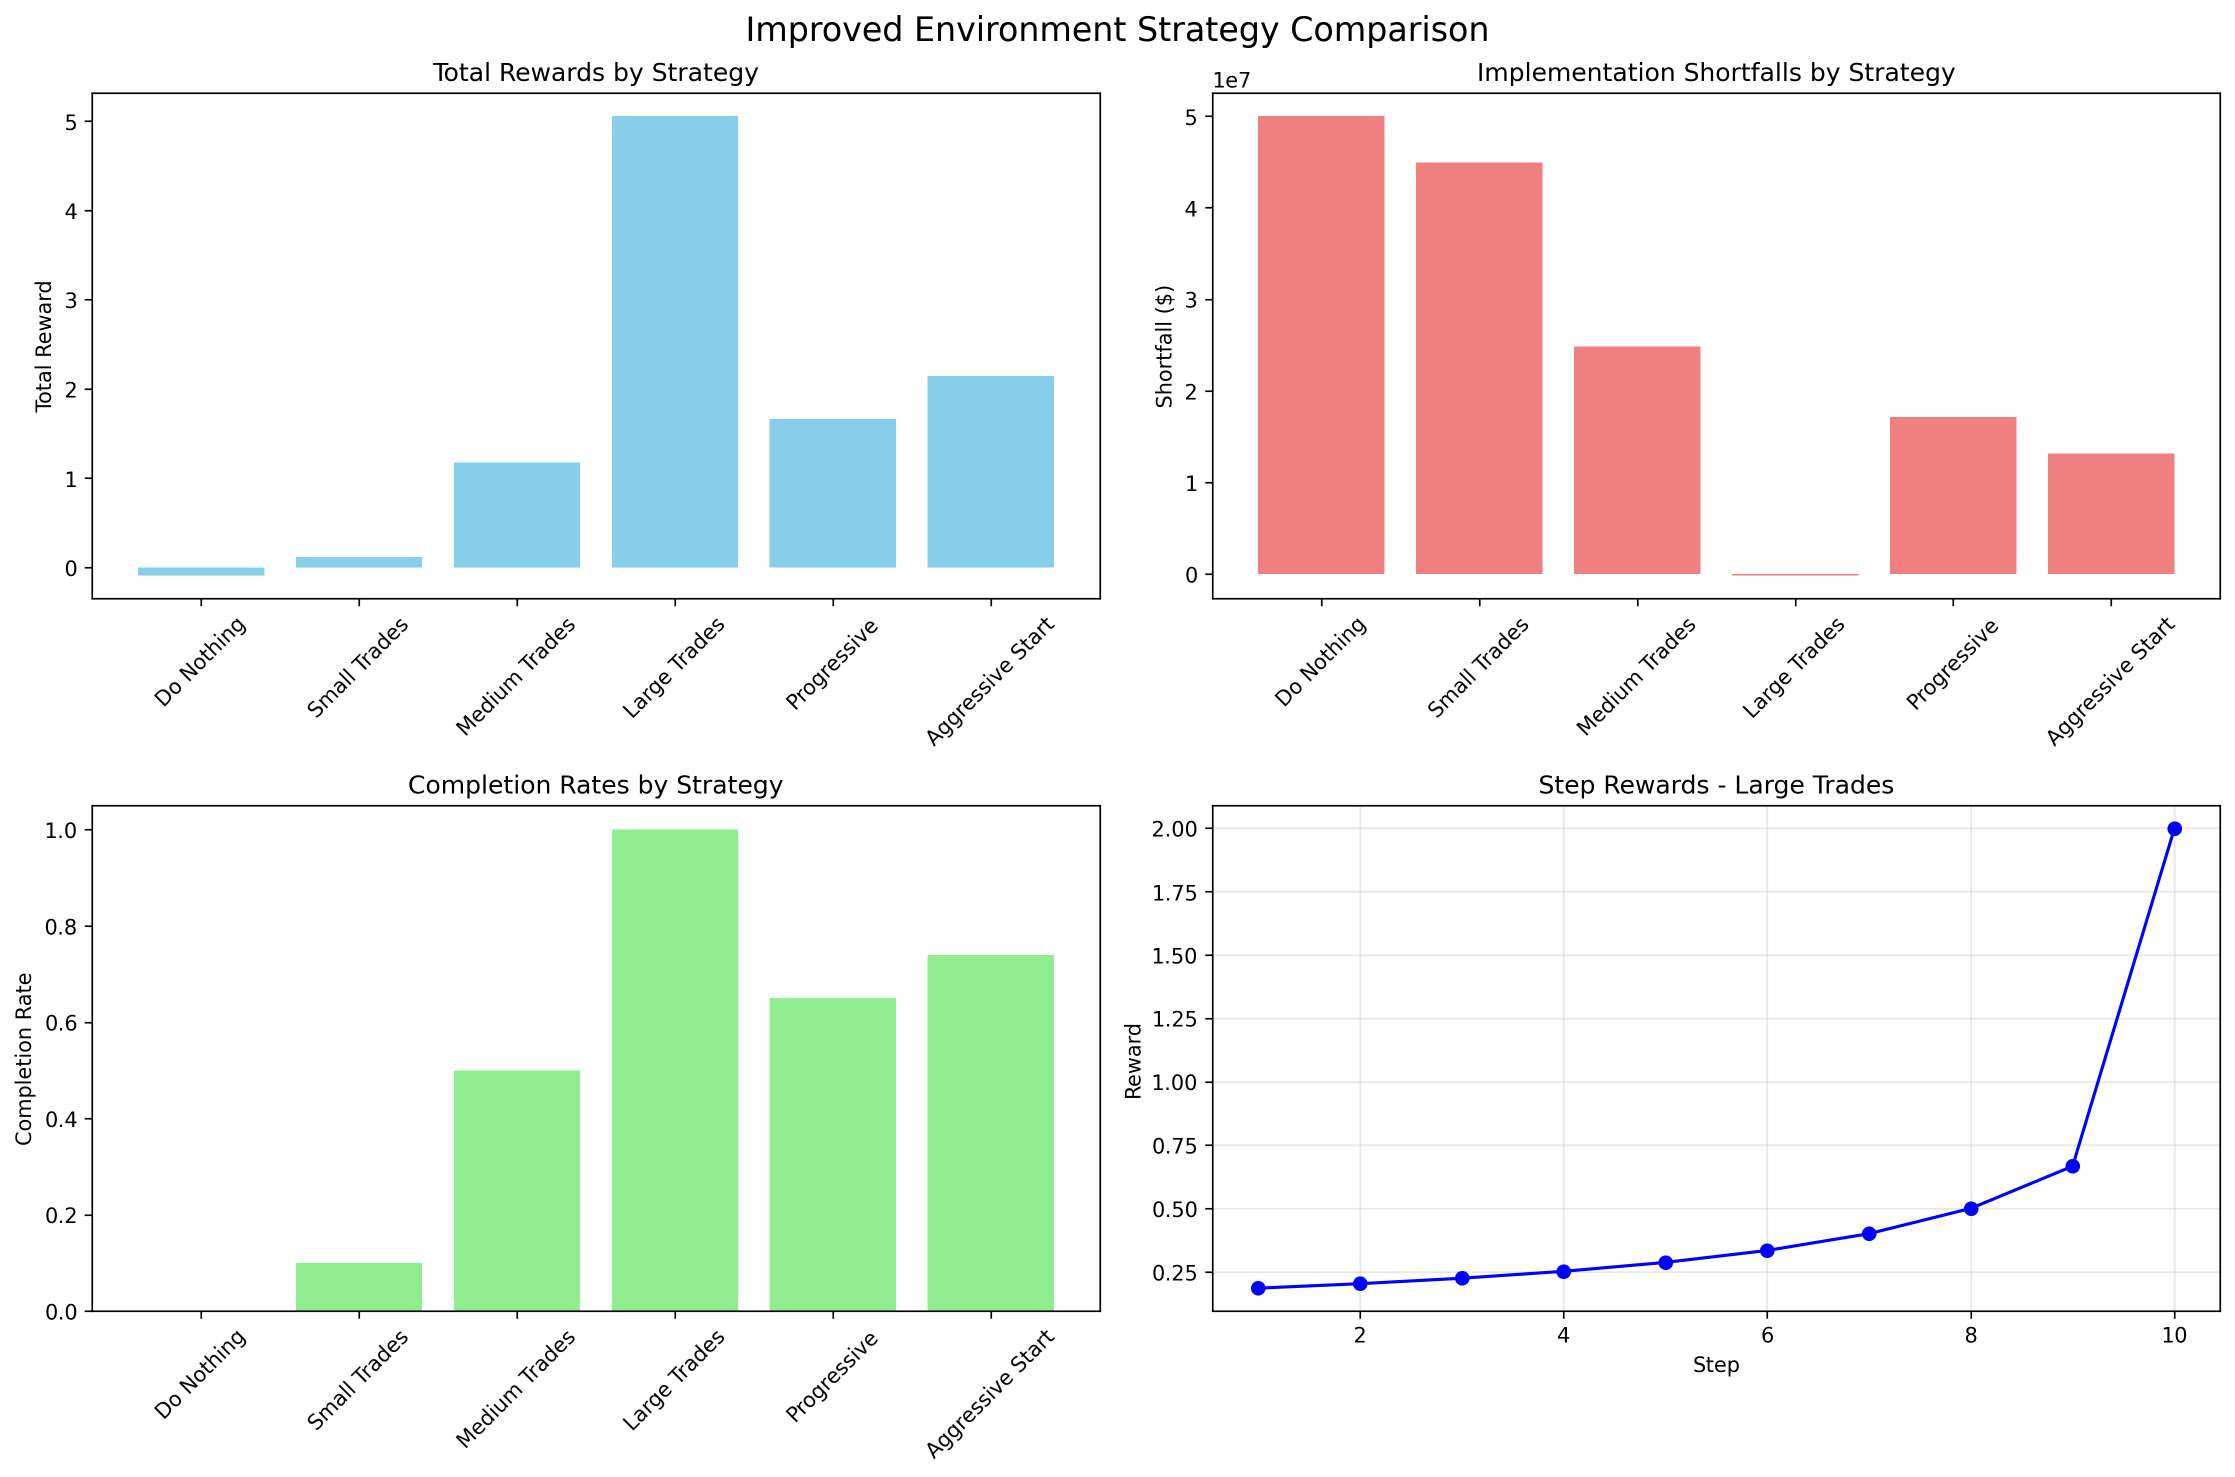
\includegraphics[width=0.6\linewidth]{improved_env_comparison.pdf}
		\caption{enhanced environment}
	\end{figure}
\end{frame}

\begin{frame}{Sparse Rewards}
	\begin{figure}[ht]
		\centering
		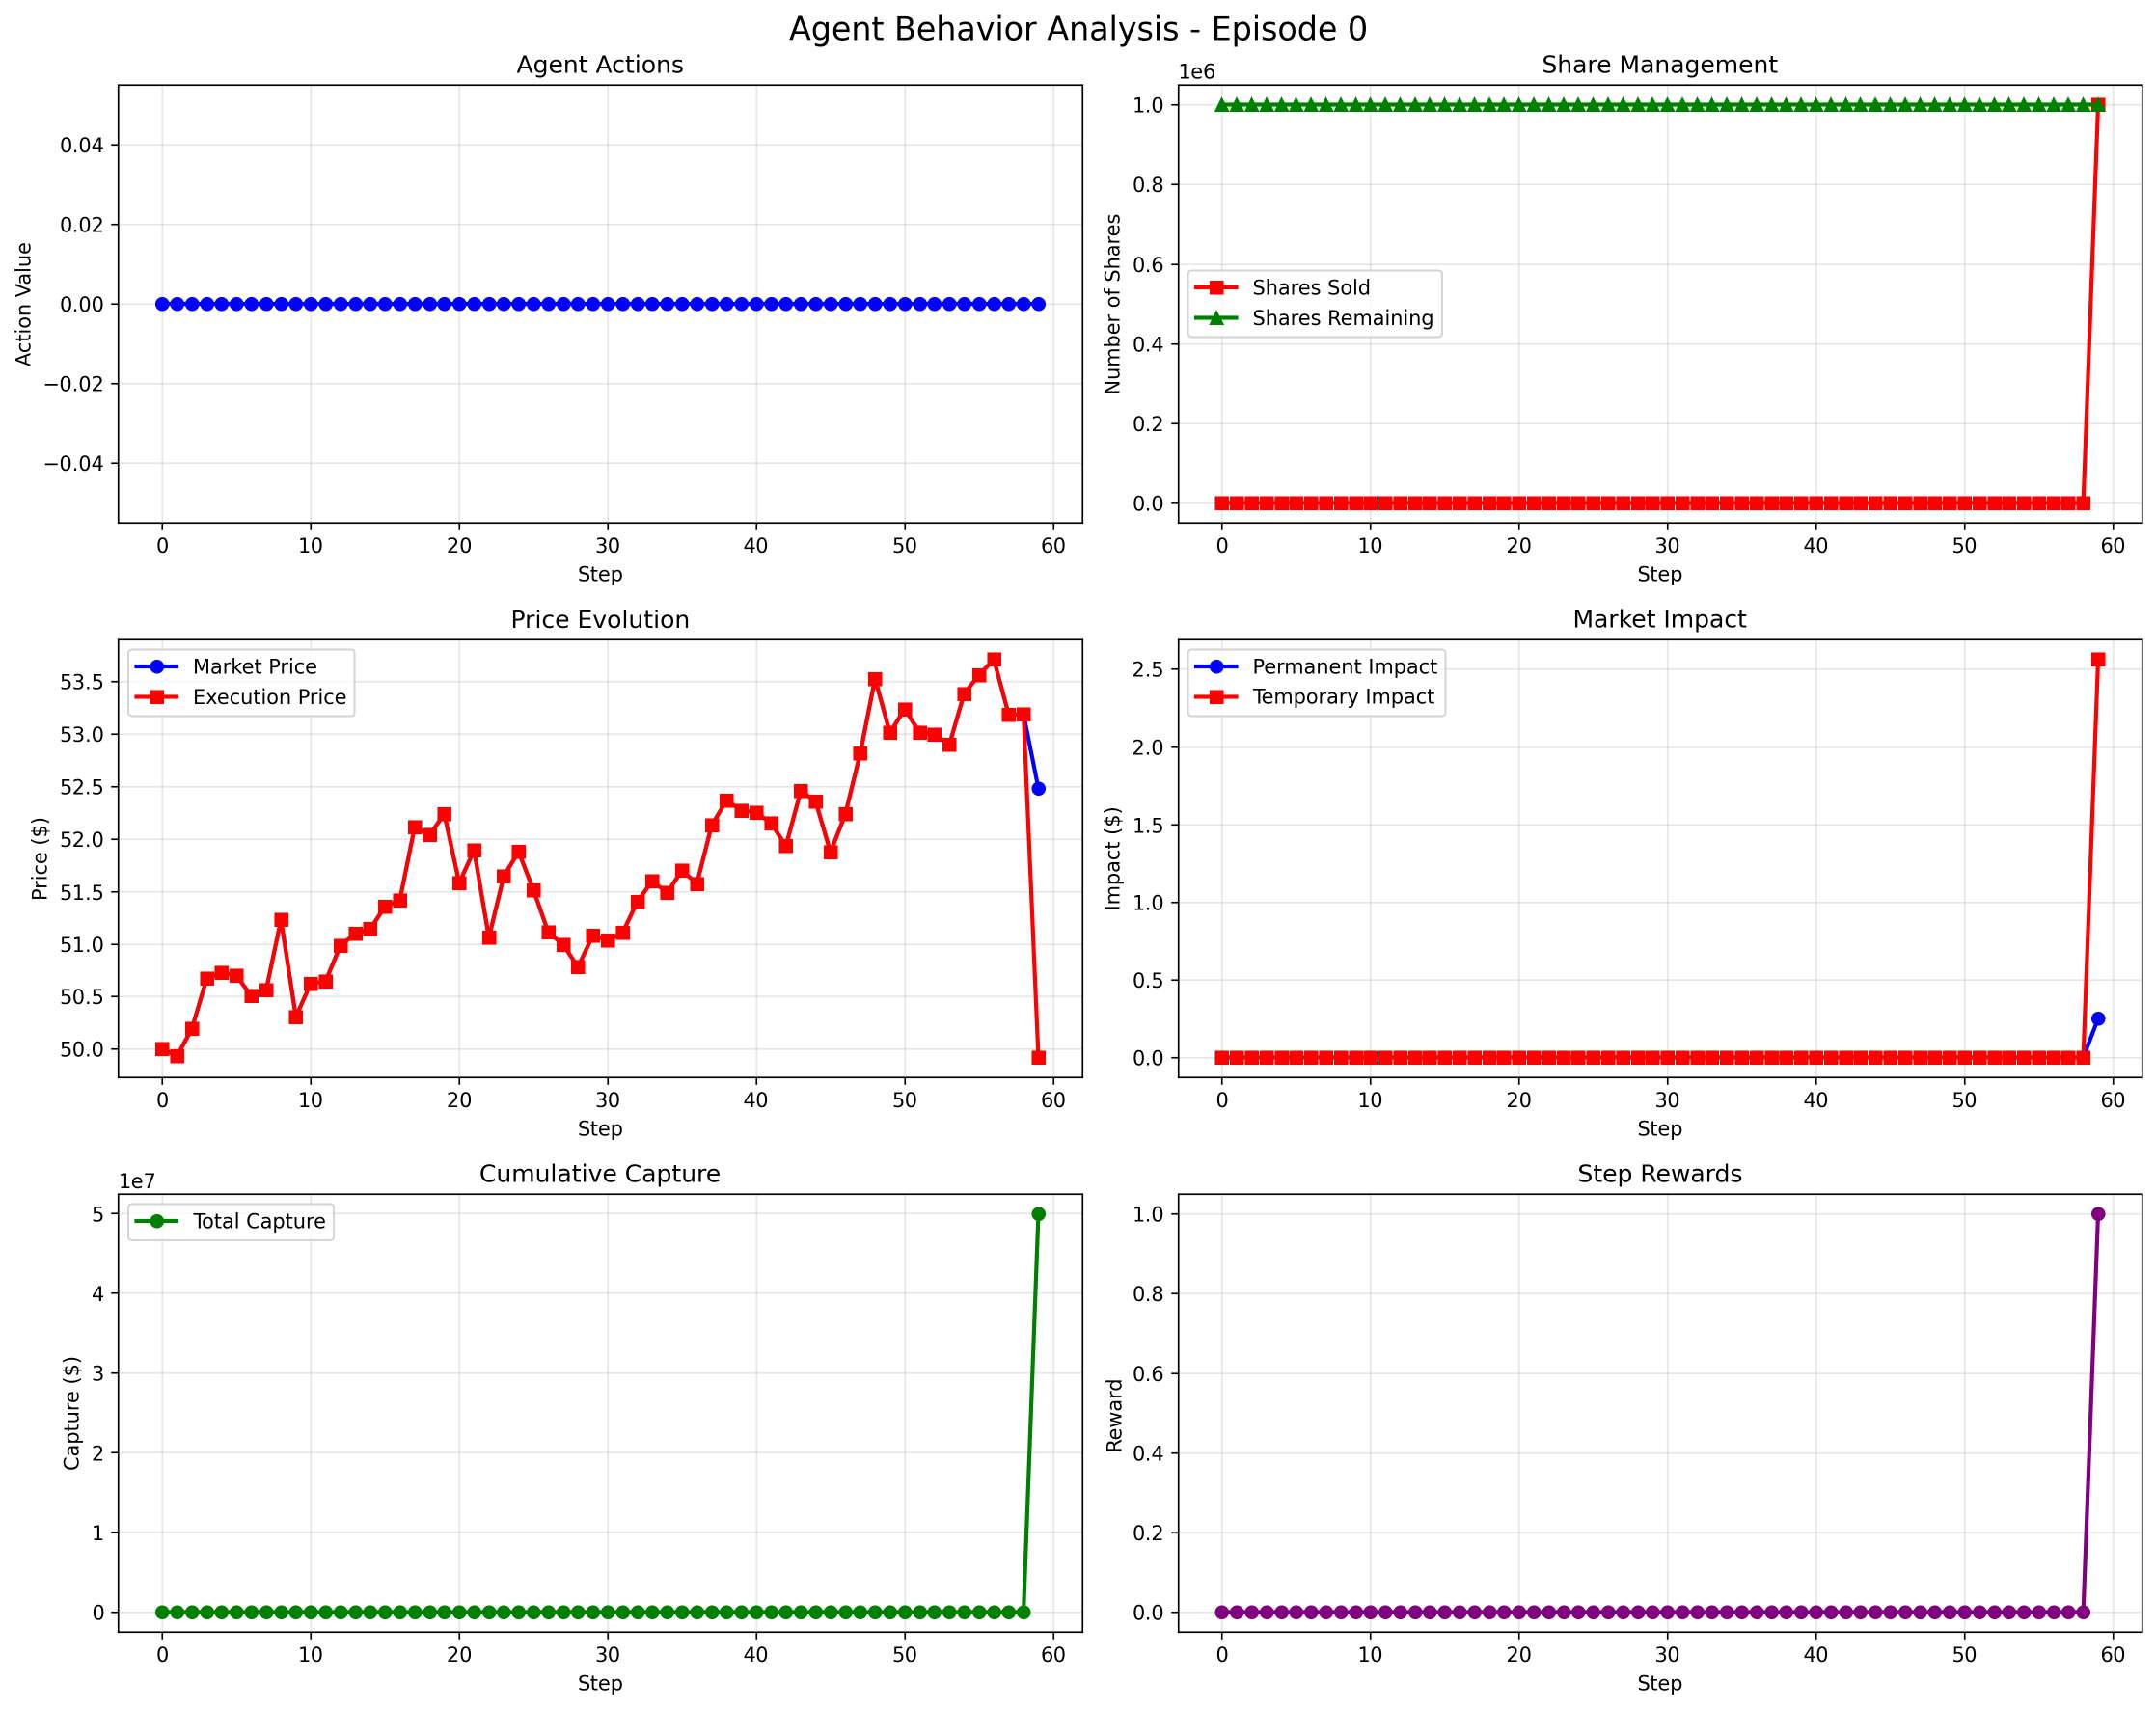
\includegraphics[width=0.6\linewidth]{agent_behavior_episode_0.pdf}
	\end{figure}
\end{frame}

\begin{frame}{Dense Rewards}
	\begin{figure}[ht]
		\centering
		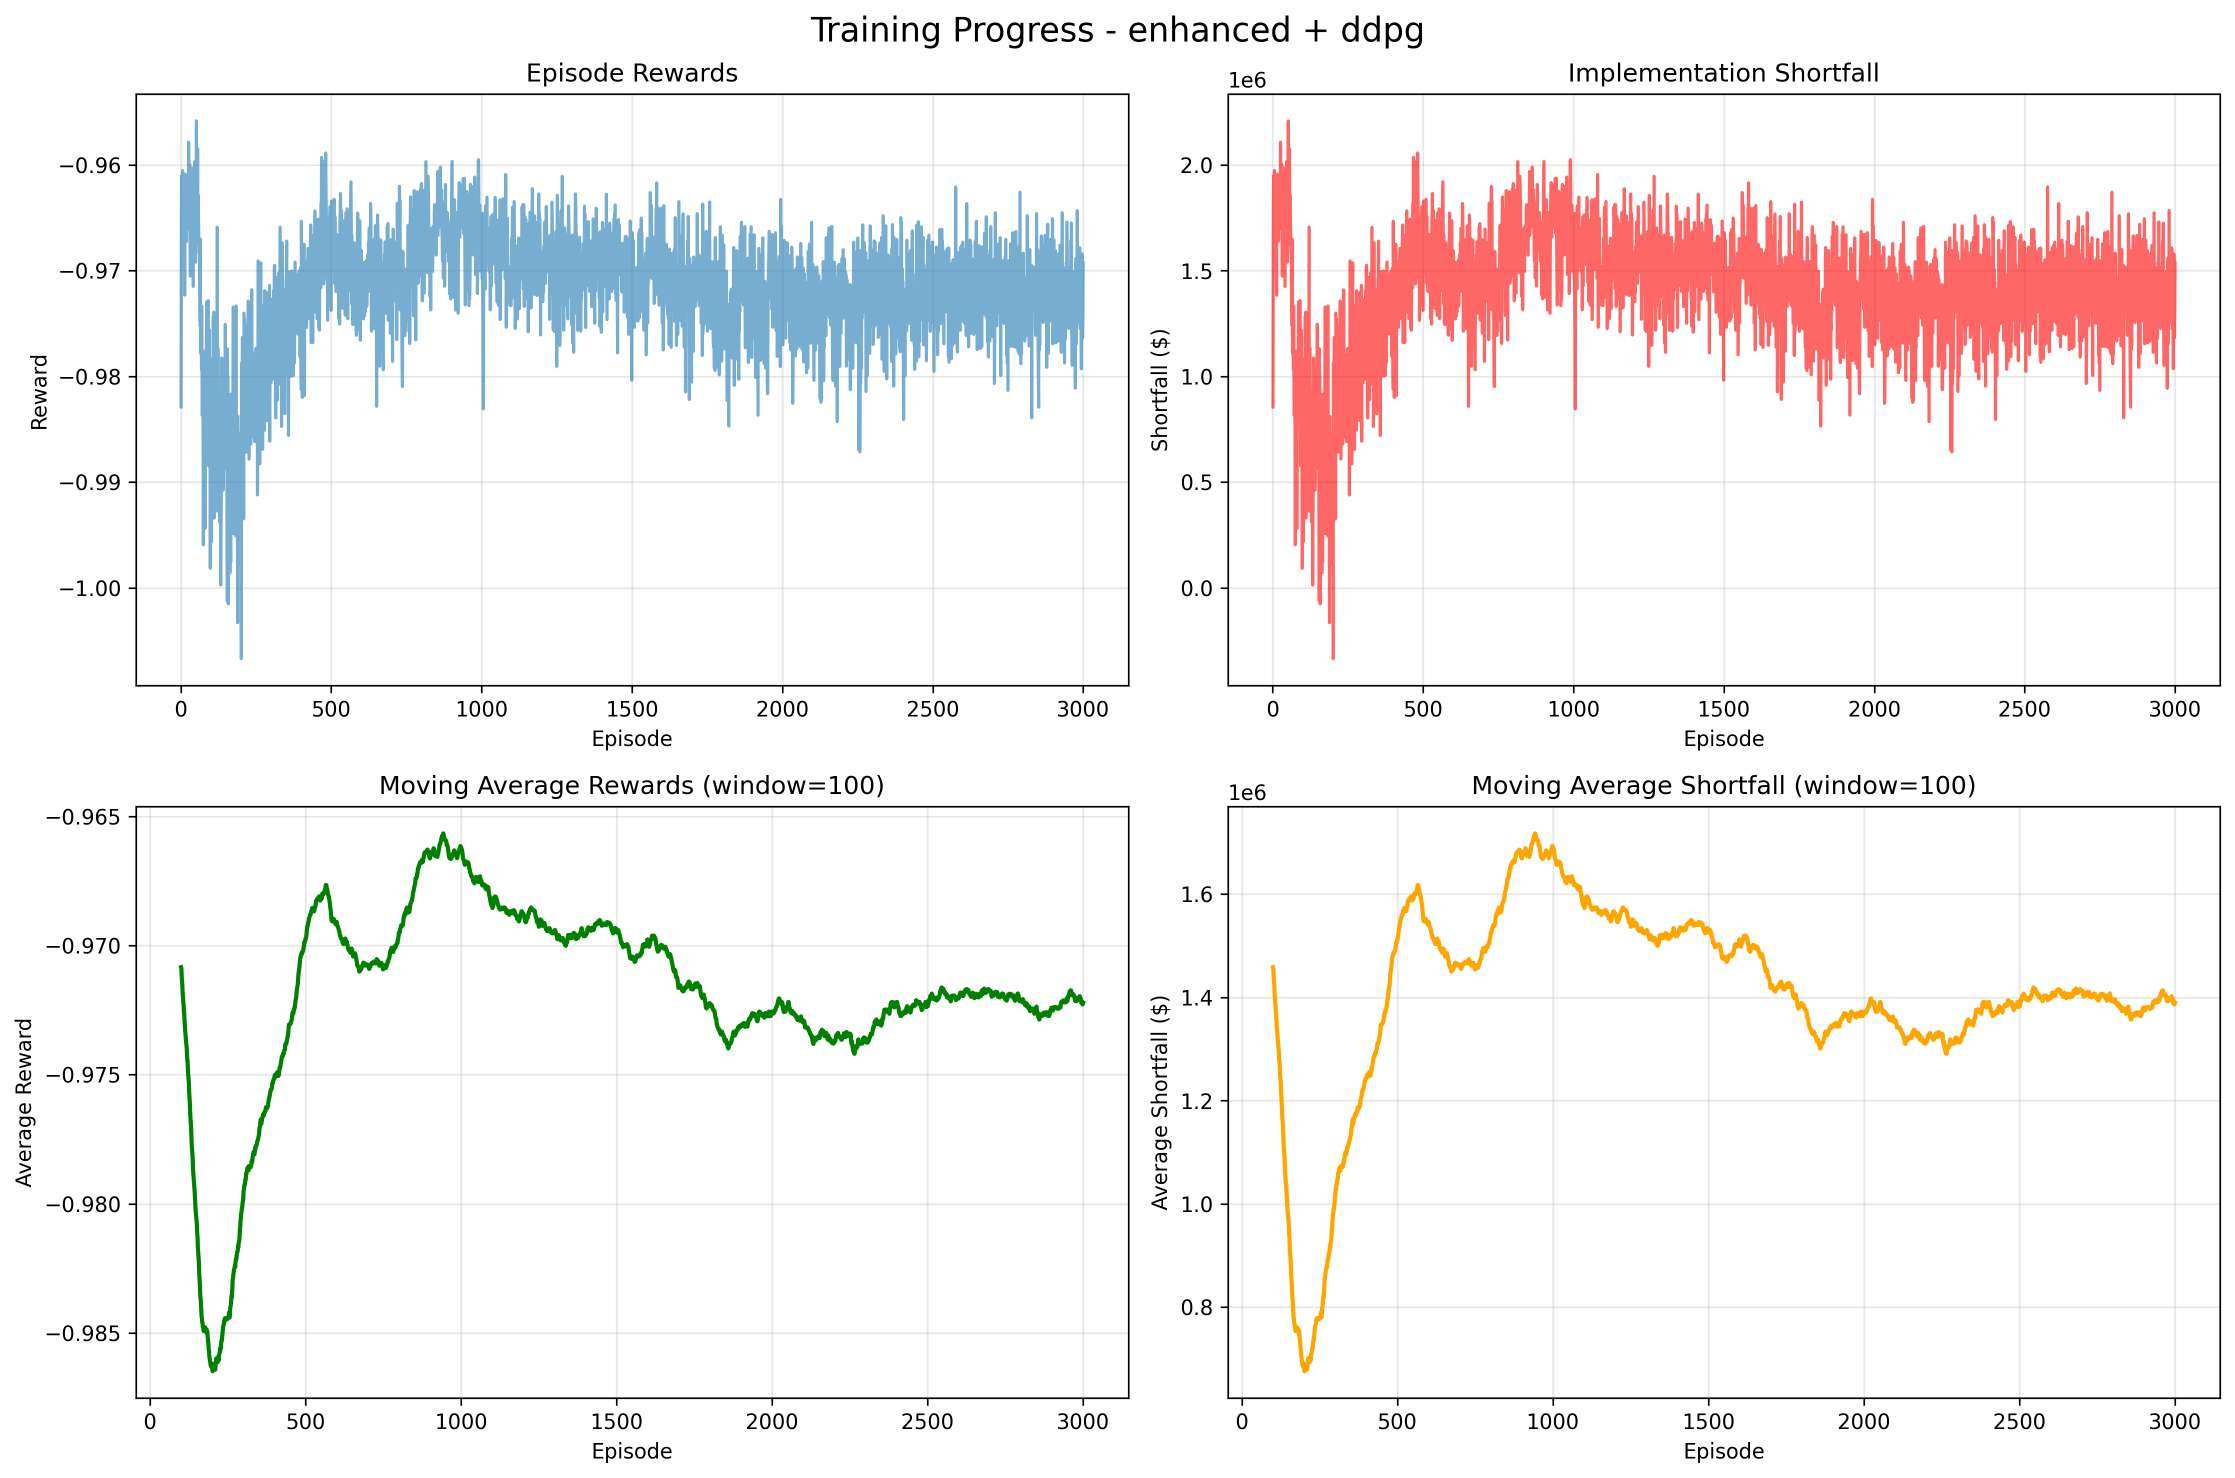
\includegraphics[width=0.6\linewidth]{training_progress_ddpg.pdf}
		\caption{ddpg dense reward training progress}
	\end{figure}
\end{frame}

\begin{frame}{Dense Rewards vs Almgren Chriss Model}
	\begin{figure}[ht]
		\centering
		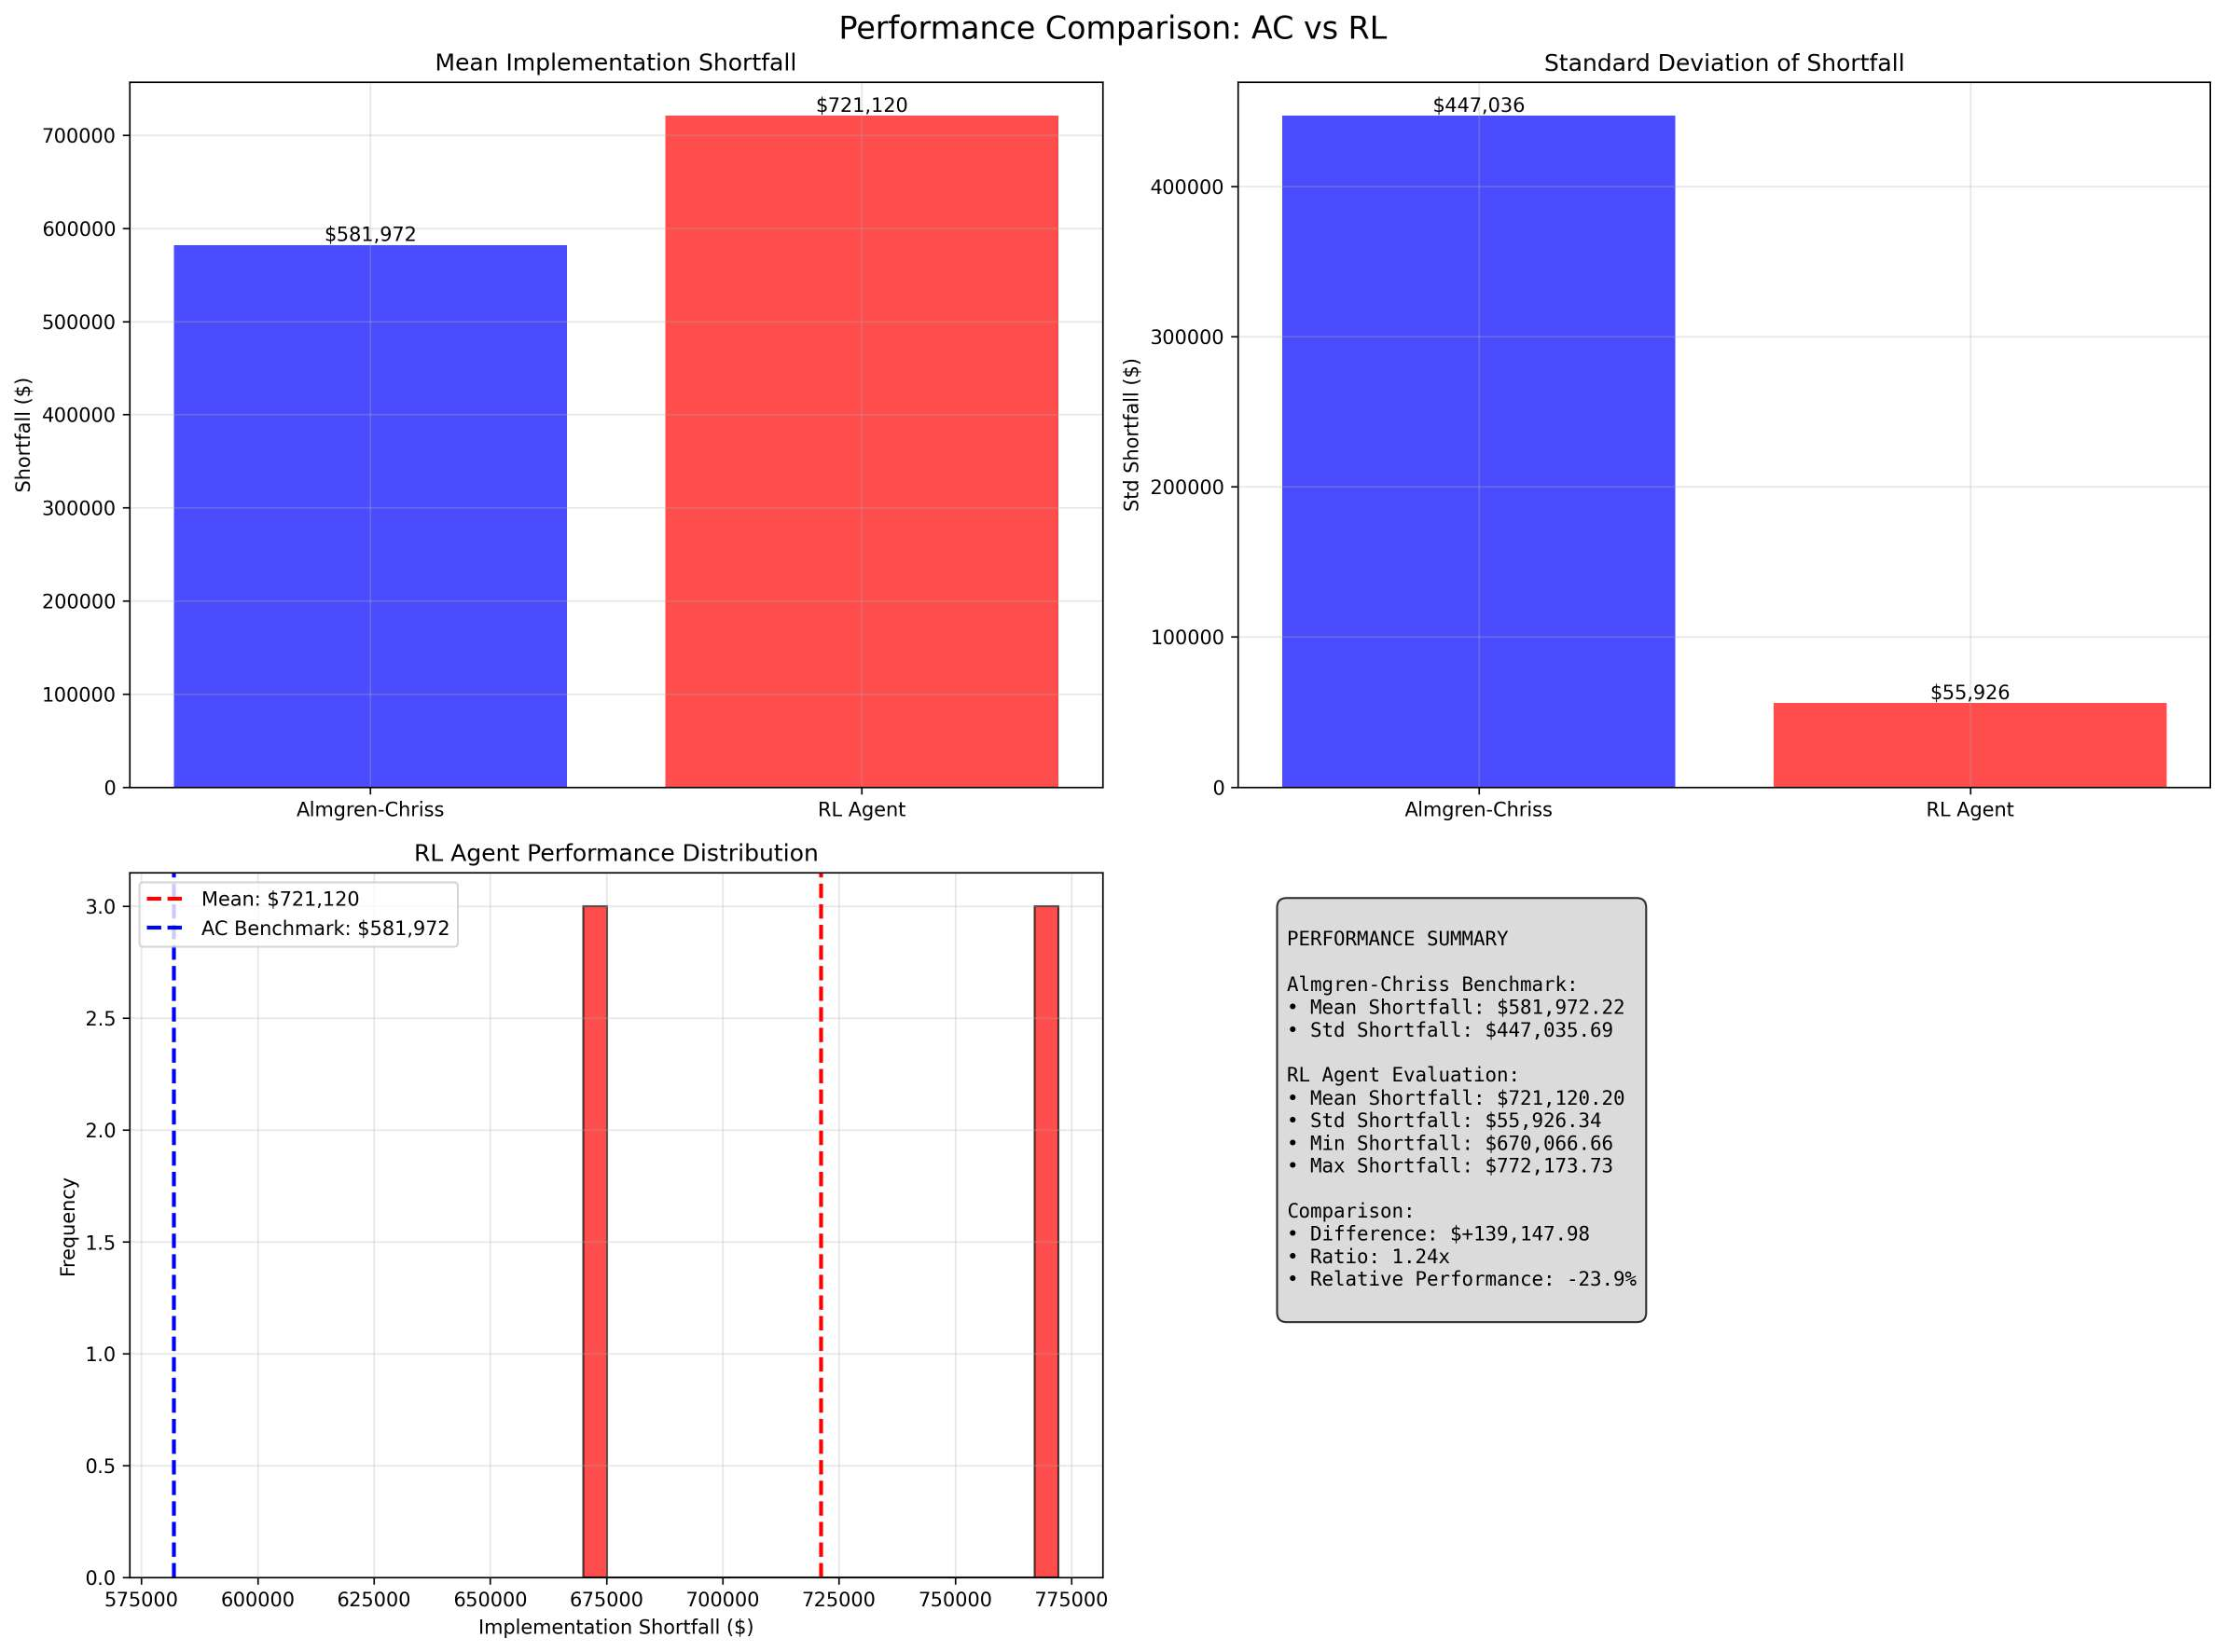
\includegraphics[width=0.6\linewidth]{performance_comparison.pdf}
		\caption{}
	\end{figure}
\end{frame}

\begin{frame}{Beyond ABM: GBM and AR($L$) Price Dynamics}
	\begin{itemize}
		\item \textbf{Arithmetic Brownian Motion (ABM):} AC’s baseline model – price changes $\Delta S$ are normal with constant variance, no memory. (Can lead to unrealistic behavior like negative prices over long horizons.)
		\item \textbf{Geometric Brownian Motion (GBM):} More realistic model: $dS_t = \mu S_t\,dt + \sigma S_t\,dW_t$. Prices evolve multiplicatively, so volatility is proportional to price and prices stay positive.
		\item \textbf{Autoregressive returns (AR($L$)):} Instead of i.i.d. returns, assume $r_{t} = \phi_1 r_{t-1} + \dots + \phi_L r_{t-L} + \varepsilon_t$. Introduces serial correlation (e.g. momentum or mean-reversion) in price movements.
		\item Real markets exhibit features like short-term momentum and volatility clustering. AR models capture the former, and can be combined with volatility models (e.g. GARCH) to capture time-varying volatility.
	\end{itemize}
\end{frame}
		
% ── Slide 1: text only ──
\begin{frame}{Impact of Changing Price Dynamics}
	\begin{itemize}
		\item \textbf{Higher volatility (GBM vs ABM):} When price volatility is proportional to price (GBM), large swings become more likely. This increases tail‑risk of not finishing in time at a good price – our CVaR‑focused agent responds by executing faster (reducing exposure), especially after volatility spikes. AC’s strategy, being fixed, cannot adjust to volatility on the fly.
		\item \textbf{Downward drift:} In a falling market ($\mu<0$), the optimal play is to sell early. The RL agent learns to \emph{front‑load} trades; AC’s analytic schedule would do the same only if it already “knew” the drift.
		\item \textbf{Upward drift / momentum:} With persistent positive returns (AR($L$) momentum) the RL agent sells more slowly to capture the up‑move, whereas AC’s static plan can’t time this.
	\end{itemize}
\end{frame}

% ── Slide 1: GBM ──
\begin{frame}{Impact of Changing Price Dynamics}
	\begin{figure}[ht]
		\centering
		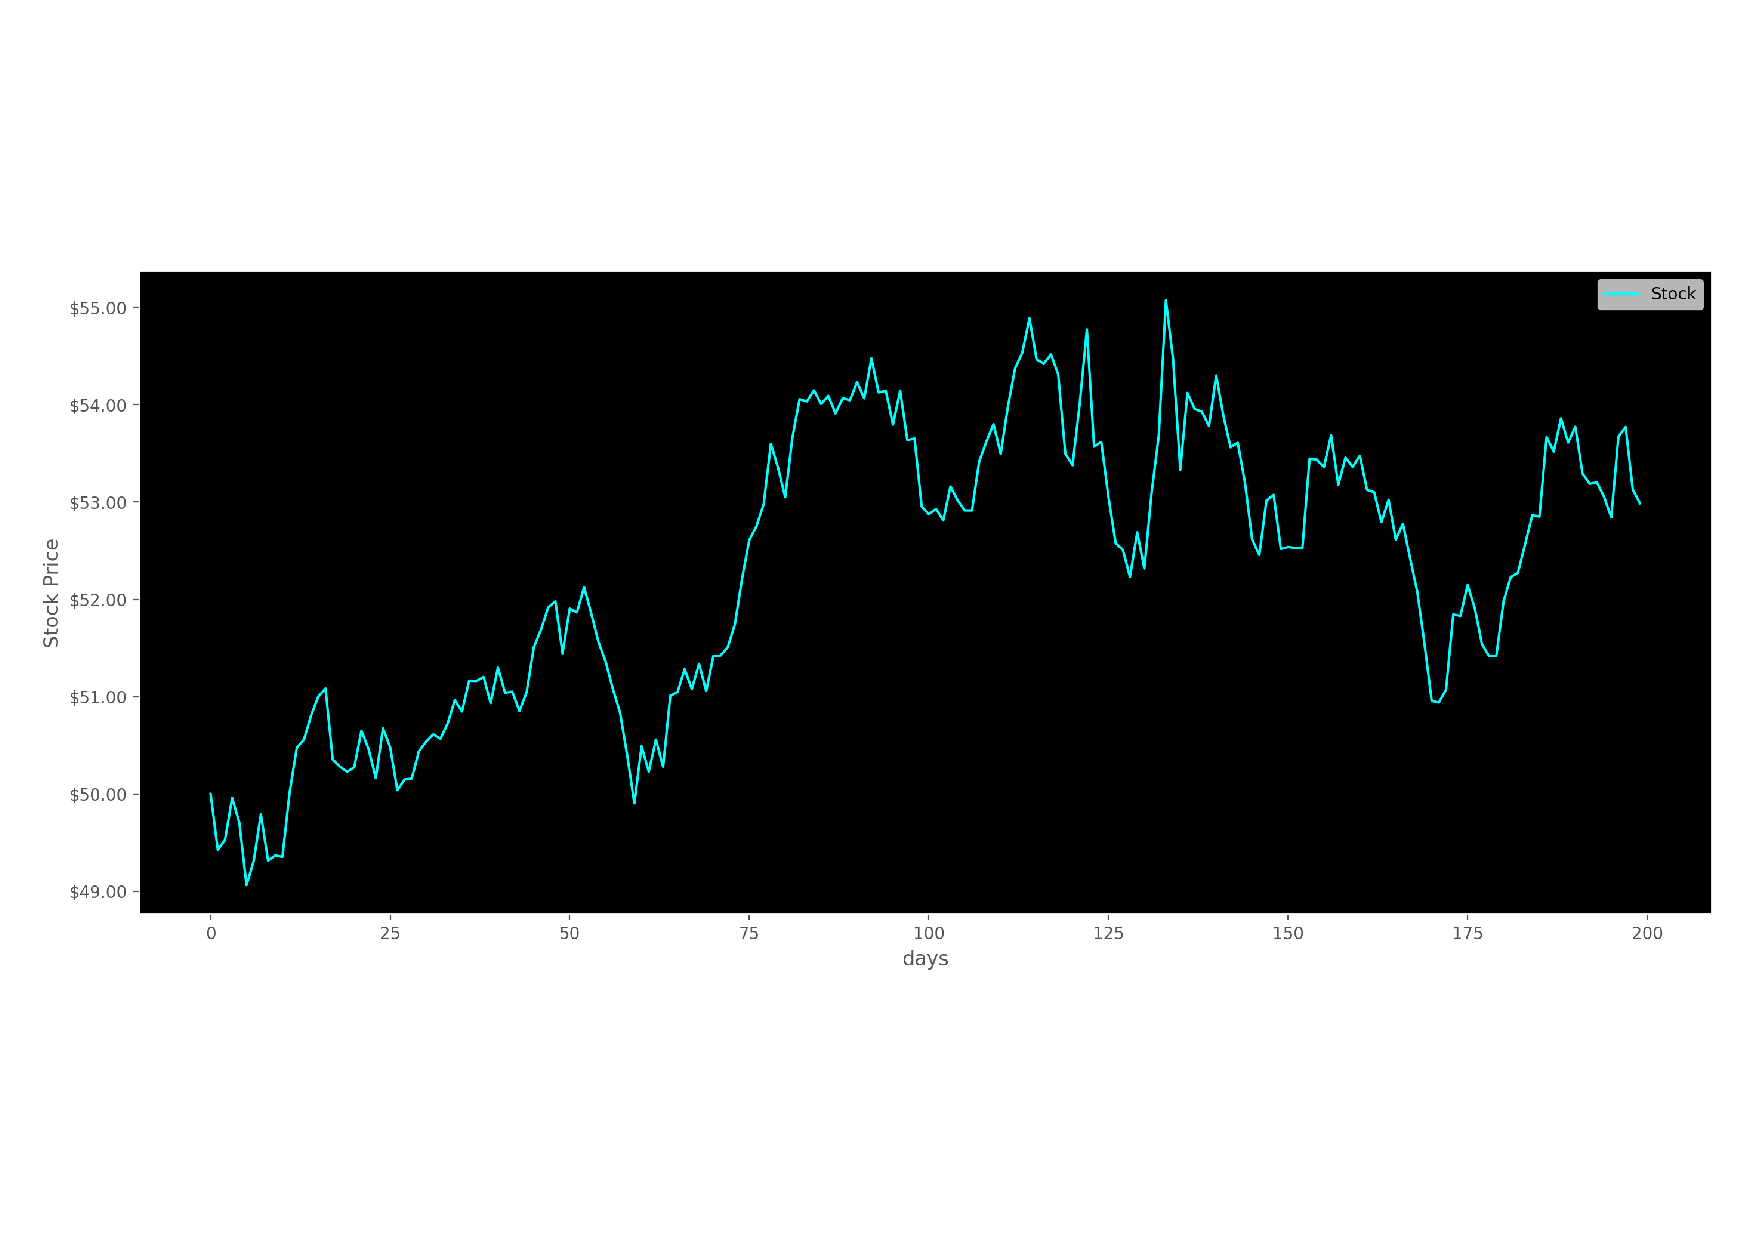
\includegraphics[width=0.8\linewidth]{gbm.pdf}
		\caption{GBM}
	\end{figure}
\end{frame}

% ── Slide 3: AR(L) ──
\begin{frame}{Impact of Changing Price Dynamics}
	\begin{figure}[ht]
		\centering
		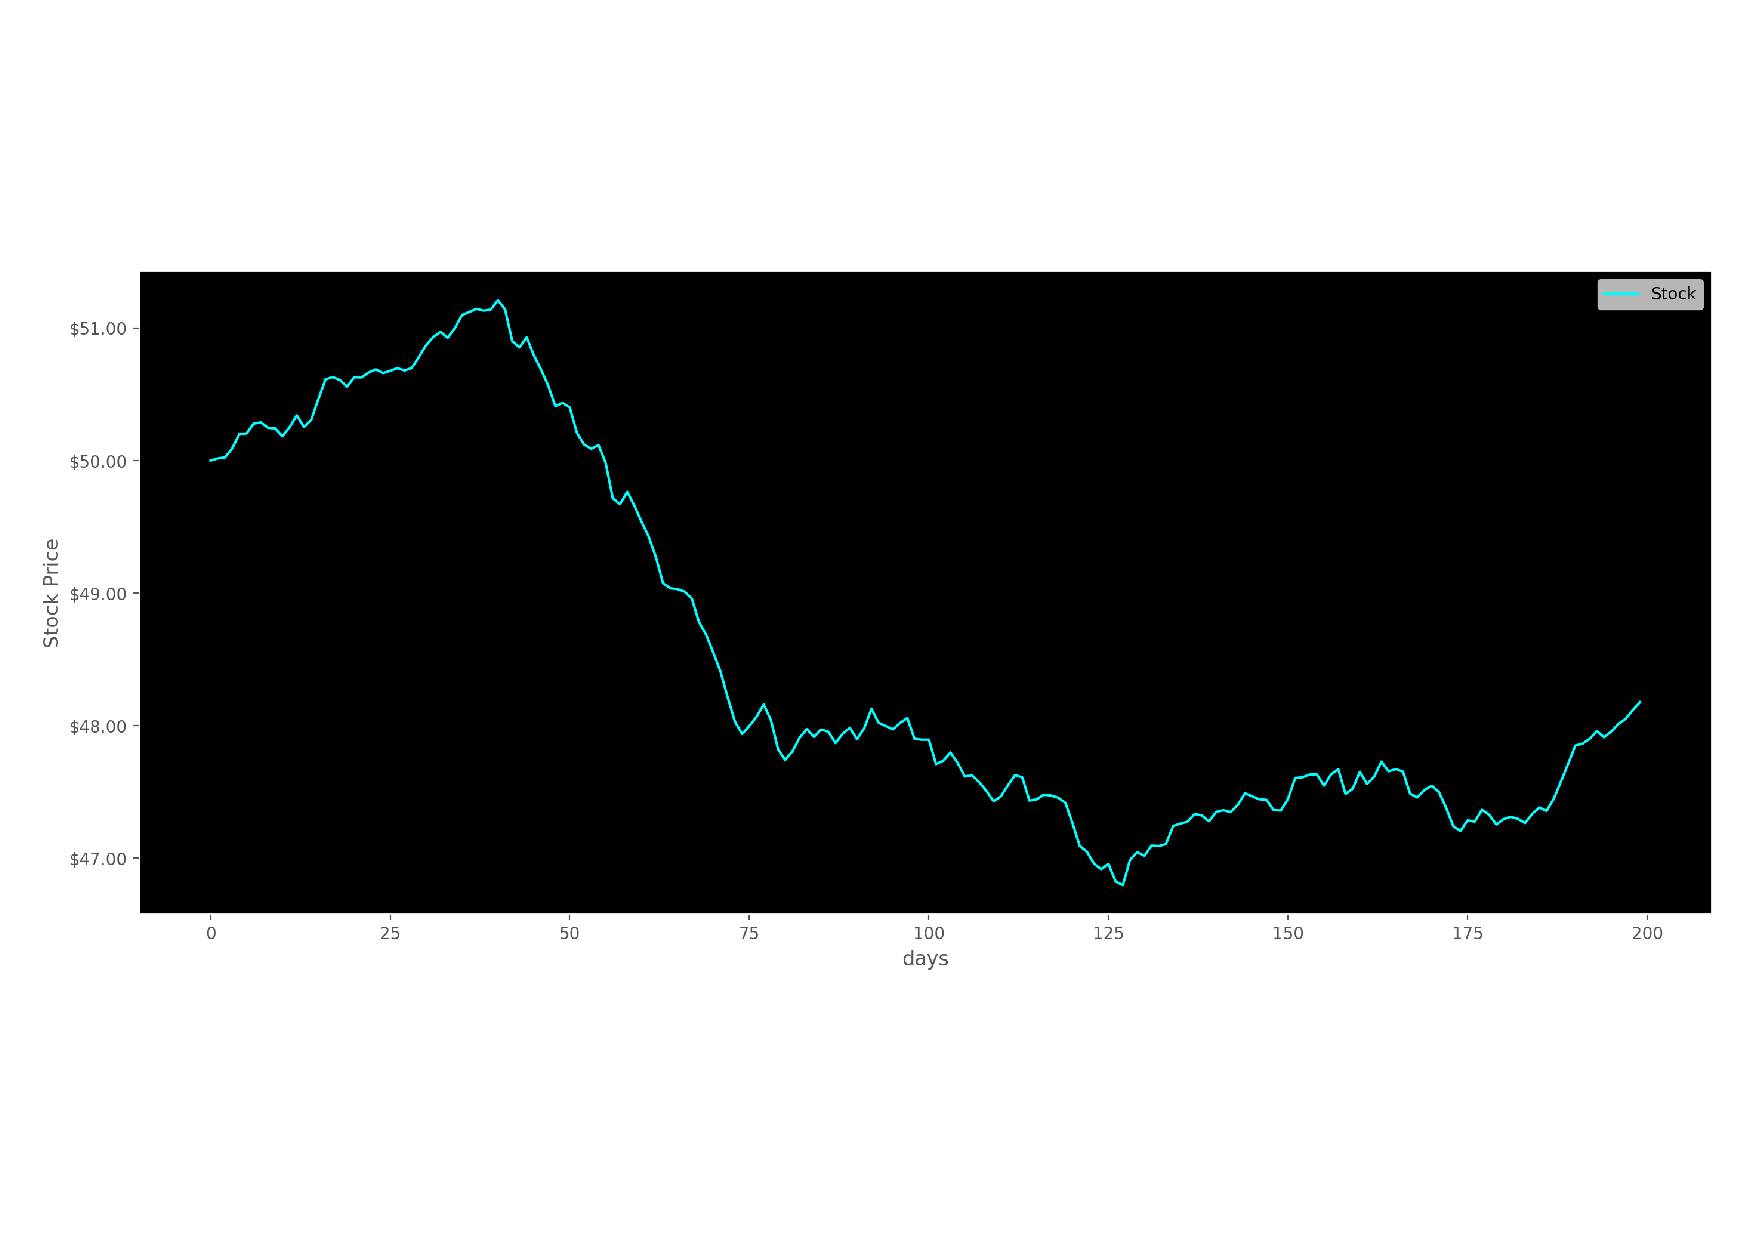
\includegraphics[width=0.8\linewidth]{arl.pdf}
		\caption{AR($L$)}
	\end{figure}
\end{frame}

		\begin{frame}{Trading Costs and Market Impact Enhancements}
			\begin{itemize}
				\item \textbf{Fixed fees:} We include a per-share cost $\epsilon$ for trading (e.g. commissions or bid-ask spread). AC’s model had a fixed cost component; we carry that over so each share sold incurs a small fixed cost.
				\item \textbf{Non-linear impact (quadratic):} In addition to linear impact, we add a term proportional to $v^2$ (square of volume traded in a single step). This models the fact that very large trades eat deeper into liquidity and incur disproportionately higher costs.
				\item \textbf{Effect on strategy:} The quadratic penalty strongly discourages large, instant trades. The agent (and even an optimized AC-like strategy) will favor spreading out the order more evenly to avoid the extra cost of big trades. Execution becomes smoother and less “impulsive.”
			\end{itemize}
			\vspace{0.5em}
		%	\todo{Show before/after utility comparison with/without non-linear cost.}
		\end{frame}
		
\begin{frame}{DDPG Baseline Performance}
	\begin{itemize}
		\item Trained a DDPG agent in the simulated environment (episodes represent full order execution). Used replay buffer of size $10^4$, batch size 128, $\gamma=0.99$, and OU noise for exploration.
		\item Convergence: the agent’s policy stabilized after sufficient training, learning to balance impact cost and risk. (Neural network: 2 hidden layers of 24 and 48 neurons in actor/critic.)
		\item Outcome vs. AC: The DDPG agent with our custom reward achieved a significantly better 95\% Expected Shortfall than the AC baseline (i.e., reduced tail-cost). \textit{Preliminary result:} ES$_{0.95}$ improved by over AC’s strategy for comparable average cost.
	\end{itemize}
\end{frame}

\begin{frame}{Performance Across Market Scenarios}
	\begin{itemize}
		\item \textbf{Simple ABM (random walk, no drift):} DDPG agent’s strategy looks similar to AC’s optimal schedule. With no predictable trends, there’s little room to improve on AC – both achieve near-optimal cost. (RL essentially “recovers” the AC solution in this regime.)
		\item \textbf{Trending market (GBM with drift):} In a market with drift, AC (if unaware of drift or unable to adapt) performs suboptimally. Our RL agent adapts: for $\mu<0$ (downtrend) it sells faster than AC, for $\mu>0$ (uptrend) it sells more slowly. This adaptability lets RL beat AC in terms of final execution cost.
		\item \textbf{Autocorrelated returns (AR($L$)):} AC’s static strategy cannot exploit short-term autocorrelation (e.g. momentum bursts or mean-reversion). The RL agent does leverage it – e.g., delaying sells during a momentum upswing or holding fire during a dip expecting a rebound – thus achieving lower cost/risk. 
		\item Overall, the more the price process deviates from AC’s assumptions (pure random walk), the larger the performance gap where RL outperforms AC.
	\end{itemize}
\end{frame}

\begin{frame}{Experiments: Action Variations}
	\begin{itemize}
		\item \textbf{Baseline Action:}  
		Sell a constant proportion of shares remaining: 
		\[
		a_k \cdot \texttt{constant\_shares\_to\_sell}
		\]
		
		\item \textbf{Spread Adjusted:}  
		Modify $a_k$ based on bid–ask spread and recent price momentum:
		\[
		a_k \cdot (1 + \texttt{spread\_factor} \cdot \texttt{momentum})
		\]
		
		\item \textbf{Volatility Adjusted:}  
		Scale $a_k$ inversely with volatility to reduce risk during high-variance periods:
		\[
		a_k \cdot \frac{\texttt{volatility}}{\texttt{daily\_price\_variation}}
		\]
		
		\item \textbf{Time Weighted:}  
		Increase execution as time runs out:
		\[
		a_k \cdot \frac{T - t_k}{T}
		\]
		
		\item \textbf{Volume Constrained:}  
		Cap execution based on a fraction of average daily volume.
		
		\item \textbf{Percent of Total Shares:}  
		Execute a fixed fraction of original shares regardless of state.
		
		\item \textbf{Rate Based:}  
		Sell shares proportional to trading speed:
		$
		a_k \cdot \frac{Q_k}{T}
		$
	\end{itemize}
\end{frame}


\begin{frame}{Experiments: Reward Variations \& Impact}
	\begin{itemize}
		\item \textbf{Reward Tuning Strategies:}
		\begin{itemize}
			\item Compared pure PnL, exponential utility, and inventory-penalizing rewards.
			\item Evaluated dense stepwise rewards vs.\ terminal-only objectives (e.g., exponential utility, CjMm).
			\item Used penalty terms for leftover inventory, large trades, and burstiness.
		\end{itemize}
		
		\item \textbf{Behavioral Effects:}
		\begin{itemize}
			\item Terminal-penalizing rewards led to earlier liquidation and smoother execution profiles.
			\item Exponential utility and CjOe reduced aggressive trading under volatility, improving stability.
			\item Inventory penalties encouraged consistent trading over time and reduced end-of-horizon pressure.
			\item Normalized rewards led to consistent behavior across assets with varying price scales.
		\end{itemize}
		
		\item \textbf{Best Configuration:}
		\begin{itemize}
			\item \textbf{CjOe + volatility-aware action mapping:} balanced cost minimization and execution consistency under noisy price dynamics.
		\end{itemize}
	\end{itemize}
\end{frame}

\begin{frame}{Optimal DDPG Average Shortfall}
	\begin{figure}[ht]
		\centering
		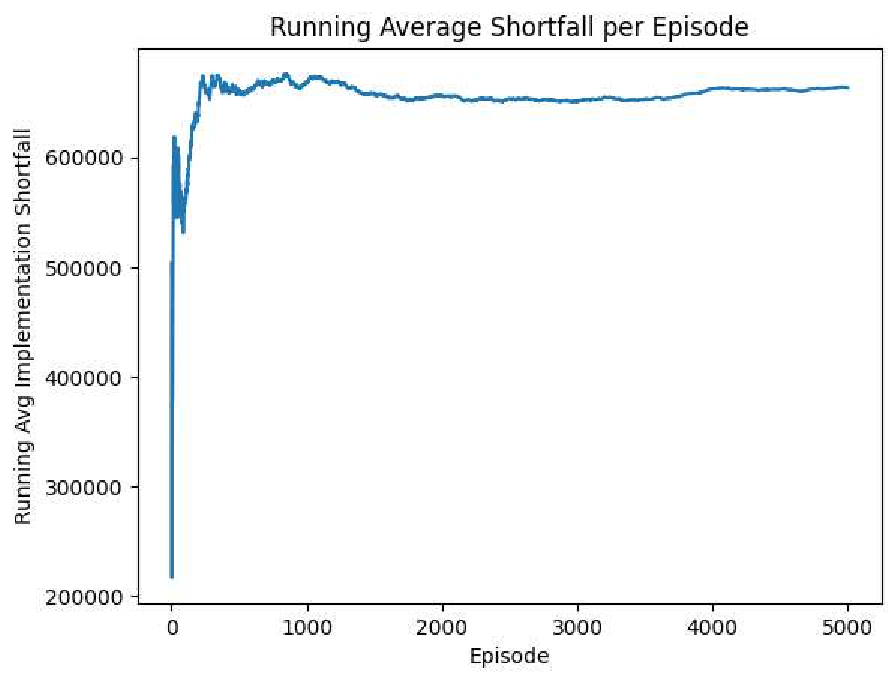
\includegraphics[width=0.55\linewidth]{DDPG_Implementation_SF_GBM.pdf}
		\caption{Average implementation shortfall of DDPG agent training in GBM environment }
	\end{figure}
\end{frame}

\begin{frame}{Optimal DDPG Reward Per Episode}
	\begin{figure}[ht]
		\centering
		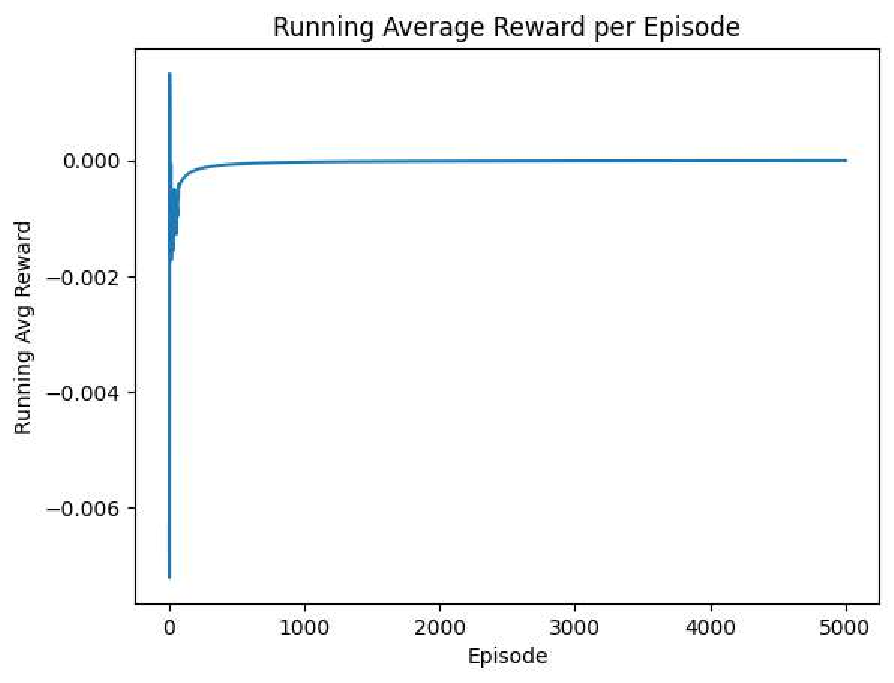
\includegraphics[width=0.55\linewidth]{DDPG_Implementation_Reward_GBM.pdf}
		\caption{Reward of DDPG agent training in GBM environment }
	\end{figure}
\end{frame}

\begin{frame}{Best DDPG Result}
	\begin{figure}[ht]
		\centering
		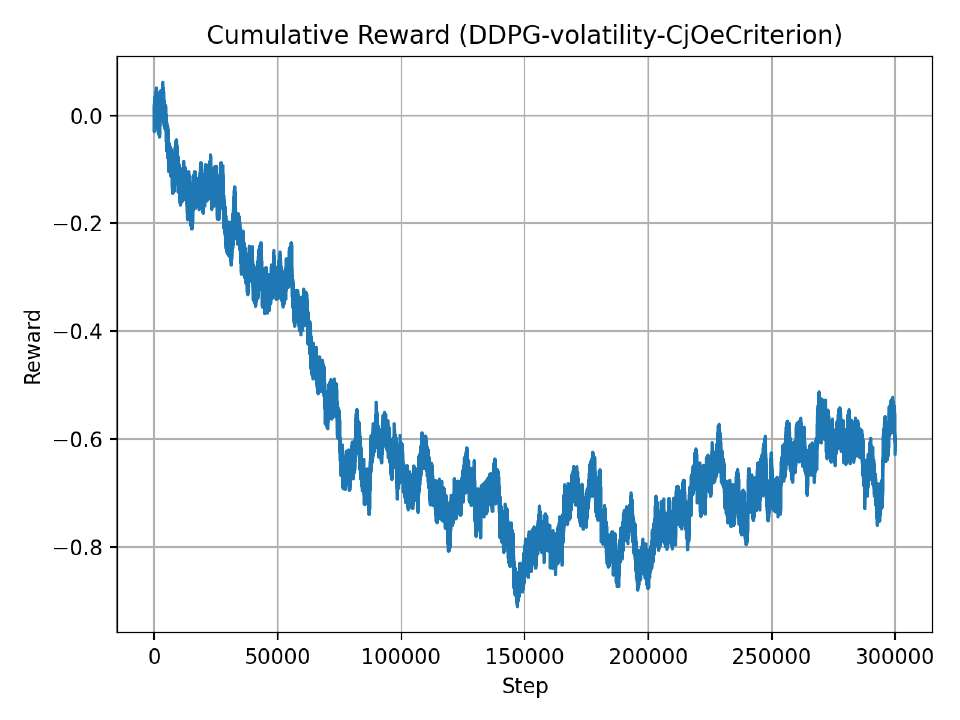
\includegraphics[width=0.55\linewidth]{cumulative_reward.pdf}
		\caption{cumulative reward of training on CjOe + volatility-aware action}
	\end{figure}
\end{frame}

\begin{frame}{DDPG test against Almgren Chriss Model}
	\begin{table}[ht]
		\centering
		\begin{tabular}{lrr}
			\hline
			\textbf{Method} & \textbf{Mean (\$)}  & \textbf{Std. Dev. (\$)} \\ 
			\hline
			Agent           &  604341.86        &   406969.01             \\ 
			AC              & 1735125.39       & 2391435.81            \\ 
			\hline
		\end{tabular}
	\end{table}
\end{frame}

\begin{frame}{Limitations of DDPG in Execution}
	\begin{itemize}
		\item \textbf{Q-value overestimation:} DDPG’s single critic can develop an optimistic bias, overestimating the value of certain actions, which may lead the policy astray (taking on more risk than intended).
		\item \textbf{Training instability:} Delicate hyperparameter tuning is needed. We observed that slight changes (learning rates, noise scale, etc.) sometimes caused divergence or very slow convergence.
		\item \textbf{Exploration challenges:} With a deterministic policy, DDPG relies on external noise for exploration. If noise is not well-tuned, the agent might not explore some strategies (risk of getting stuck in a local optimum strategy that’s suboptimal globally).
		\item \textbf{Sample inefficiency:} DDPG can require a lot of training episodes to reliably learn a good policy (especially with a sparse reward). This could be an issue if using limited real-market data for learning.
	\end{itemize}
\end{frame}

\begin{frame}{TD3: Twin-Delayed DDPG}
	\begin{itemize}
		\item \textbf{Twin Critic Networks} — two $Q$’s to {\small$\min$} over, cuts bias  
		\item \textbf{Target Policy Smoothing} — add small noise to target action  
		\item \textbf{Delayed Actor Updates} — update policy every $d$ critic steps  
		\item \textbf{Pros vs.\ DDPG:}
		\begin{itemize}
			\item Far more stable learning  
			\item Dramatically reduces over-optimistic value estimates  
		\end{itemize}
		\item \textbf{Trade-off:} Slightly more compute (two critics), but same replay buffer  
	\end{itemize}
\end{frame}

\begin{frame}{Twin Delayed DDPG (TD3)}
	\begin{itemize}
		\item \textbf{Twin Critics:} TD3 uses two critic networks $Q_1, Q_2$ and takes the minimum $Q$ value for actor updates and target calculations. This “double Q-learning” approach reduces overestimation bias.
		\item \textbf{Delayed Policy Updates:} The actor (policy) network in TD3 is updated less frequently (e.g. every 2 or 3 critic updates). This ensures the critic values are more stable and reliable when the actor learns, preventing unstable oscillations.
		\item \textbf{Target Policy Smoothing:} When computing the target $Q$ values for the critic, TD3 adds a small random noise to the target action (clipped to avoid extremes). This makes the critic target more robust, preventing the policy from exploiting sharp local peaks in $Q$.
		\item \textbf{Effect:} TD3 provides much more stable training than vanilla DDPG. In our context, it means the agent’s learning curve is smoother and less prone to sudden divergence. It achieves equal or better execution performance, but with more reliable convergence.
	\end{itemize}
\end{frame}

\begin{frame}{Soft Actor–Critic (SAC)}
	\begin{itemize}
		\item \textbf{Maximum-Entropy Objective:}
		\[
		J(\pi)=\sum_{t}\gamma^t\Bigl[r(s_t,a_t)+\alpha\,\mathcal{H}\bigl(\pi(\cdot|s_t)\bigr)\Bigr]
		\]
		\item Learns a \emph{stochastic} Gaussian policy $\pi_\phi(a|s)$
		\item Twin critics + entropy bonus → robust value estimates
		\item Auto-tunes temperature $\alpha$ to achieve desired entropy
		\item \textbf{Pros:}
		\begin{itemize}
			\item Built-in exploration bonus  
			\item Very stable under stochastic rewards  
			\item State-of-the-art in many continuous tasks  
		\end{itemize}
		\item \textbf{Cons:} More networks \& hyperparameters (but auto-tuning helps)
	\end{itemize}
\end{frame}

\begin{frame}{Soft Actor-Critic (SAC)}
	\begin{itemize}
		\item \textbf{Stochastic policy:} SAC’s actor outputs a probability distribution (e.g. Gaussian) over actions, and actions are sampled from it. This inherent randomness encourages exploration and learning a distribution of good actions.
		\item \textbf{Maximum entropy objective:} SAC doesn’t just maximize expected reward – it also maximizes entropy (randomness) of the policy. It aims to find a policy that earns high reward \emph{while being as random as possible}. This leads to more robust, exploratory behavior.
		\item \textbf{Twin critics \& auto temperature:} Like TD3, SAC uses two critic networks to reduce bias. It also introduces a temperature parameter $\alpha$ to weight the entropy term; SAC can automatically tune $\alpha$ to balance exploration vs. exploitation.
		\item \textbf{Benefits:} In our problem, SAC’s entropy-driven approach means the agent learns not just a single deterministic strategy, but a distribution of strategies (useful under uncertainty). Training is very stable. SAC can achieve comparable or better performance than TD3, with the bonus of a naturally stochastic policy (which can be advantageous to avoid predictable execution patterns).
	\end{itemize}
\end{frame}

\begin{frame}{Implementing TD3 and SAC}
	\begin{itemize}
		\item \textbf{Unified Framework:} Both TD3 and SAC were built on the same infrastructure as DDPG.
		\begin{itemize}
			\item Identical state space, action space, and architecture.
			\item Enables direct comparisons under the same environments and reward functions.
		\end{itemize}
		\item \textbf{Shared Hyperparameters:}
		\begin{itemize}
			\item Same learning rates, batch sizes, replay buffer settings, and episode lengths.
			\item Maintains fairness across algorithmic comparisons.
		\end{itemize}
	\end{itemize}
\end{frame}
\begin{frame}{TD3: Twin Delayed DDPG}
	\begin{itemize}
		\item \textbf{Core Modifications over DDPG:}
		\begin{itemize}
			\item Two critic networks for bias reduction.
			\item Actor updates delayed: once every 2 critic updates.
			\item Target policy smoothing: Gaussian noise added to target actions during critic target computation.
		\end{itemize}
		\item \textbf{Outcomes:}
		\begin{itemize}
			\item More stable training curves than DDPG.
			\item Slight improvement in both shortfall and variance.
		\end{itemize}
	\end{itemize}
\end{frame}

\begin{frame}{Best TD3 Result}
	\begin{figure}[ht]
		\centering
		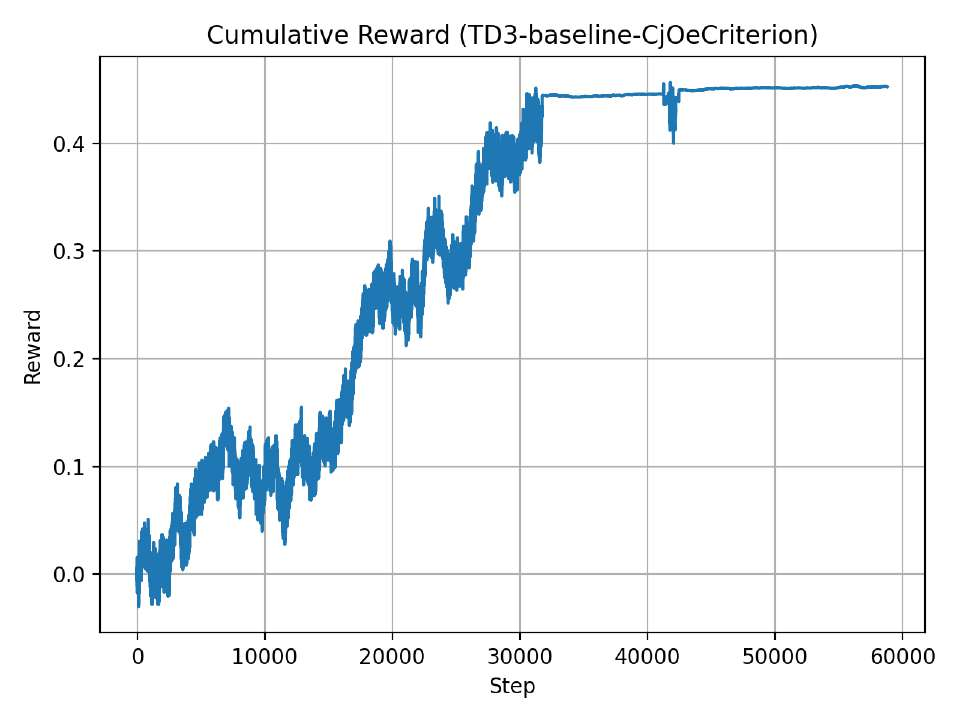
\includegraphics[width=0.55\linewidth]{td3_cumulative_reward.pdf}
		\caption{TD3 training results}
	\end{figure}
\end{frame}

\begin{frame}{Best TD3 Result}
	\begin{figure}[ht]
		\centering
		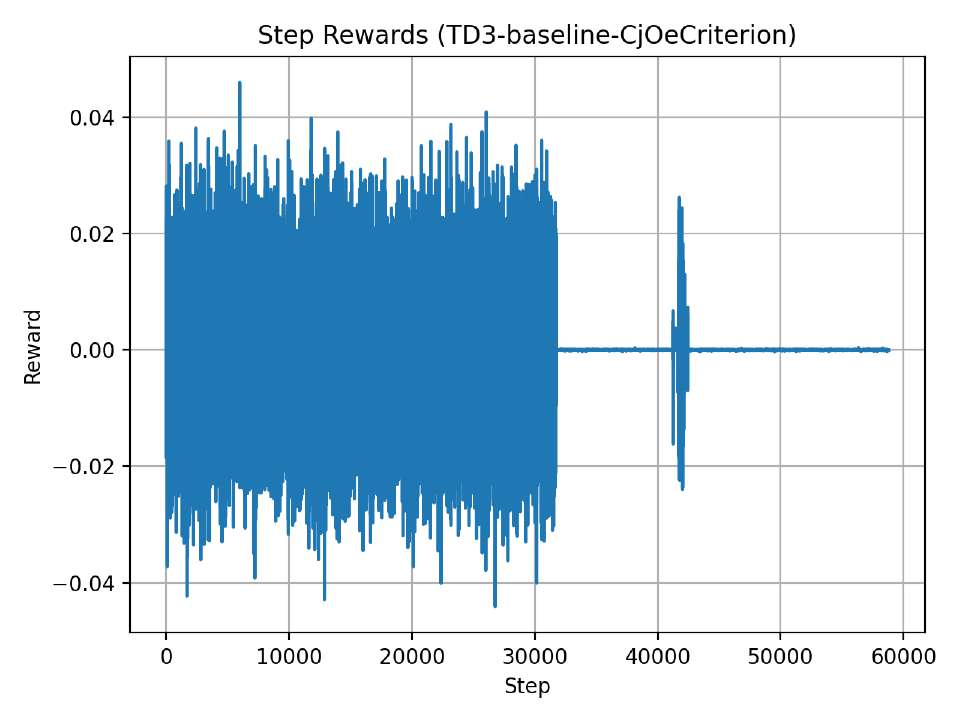
\includegraphics[width=0.55\linewidth]{step_rewards.pdf}
		\caption{TD3 training results}
	\end{figure}
\end{frame}

\begin{frame}{Best TD3 Result}
	\begin{figure}[ht]
		\centering
		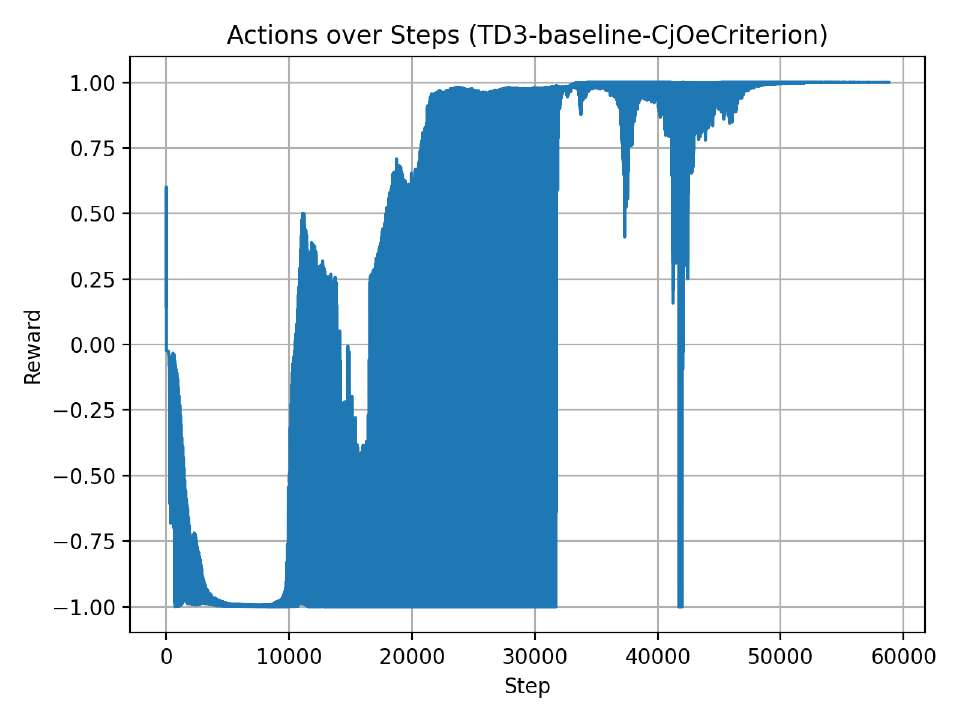
\includegraphics[width=0.55\linewidth]{actions.pdf}
		\caption{TD3 training results}
	\end{figure}
\end{frame}

\begin{frame}{TD3 Training Result}
	\begin{figure}[ht]
		\centering
		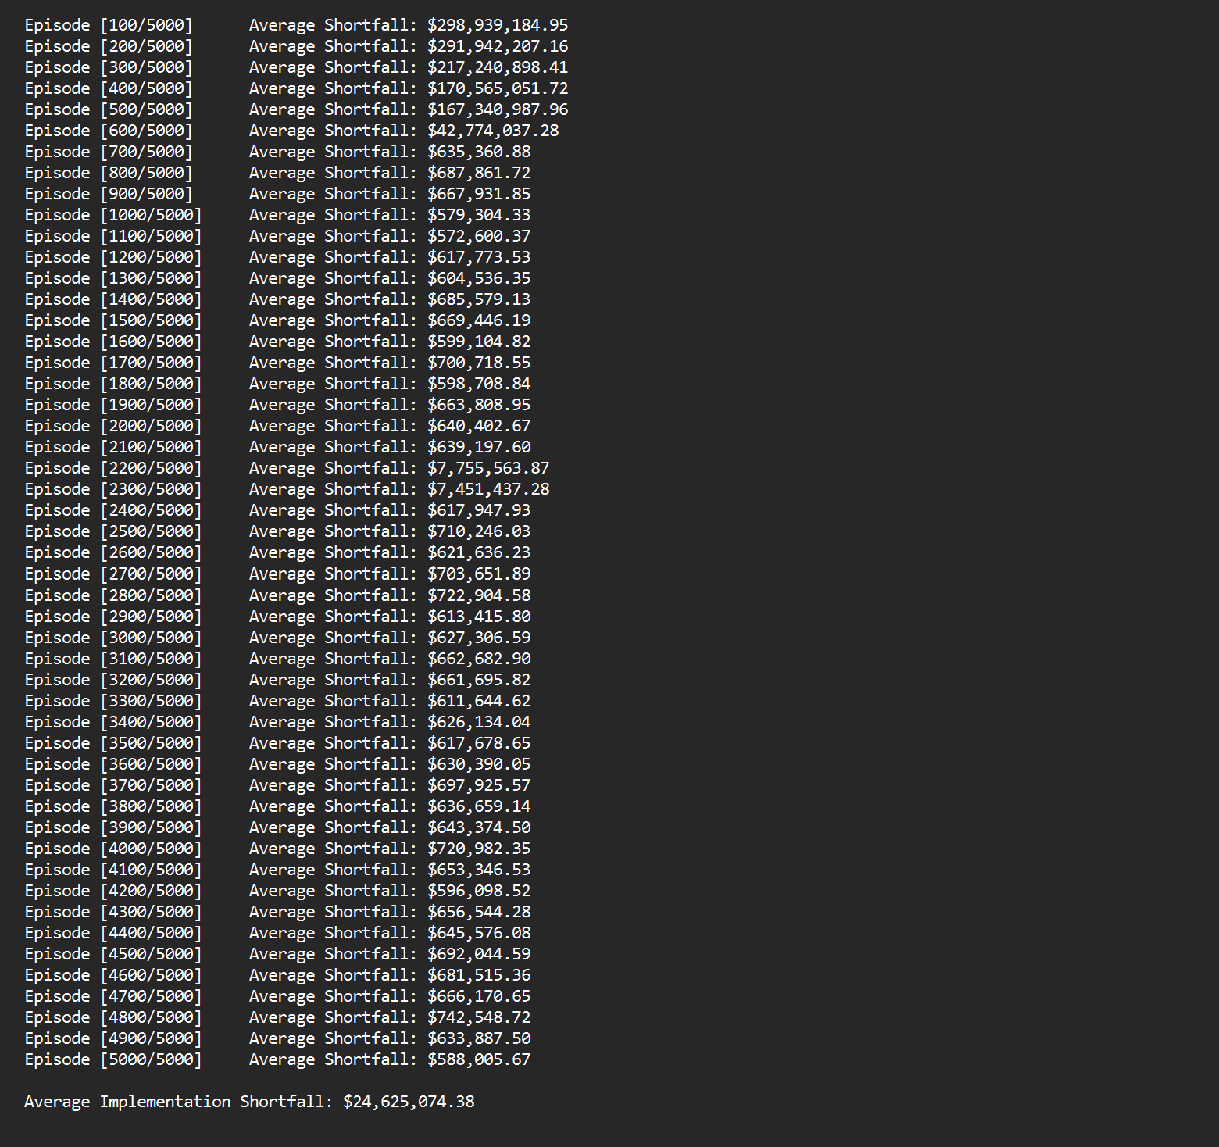
\includegraphics[width=0.4\linewidth]{training_td3.pdf}
		\caption{TD3 training average implementation shortfall}
	\end{figure}
\end{frame}

\begin{frame}{TD3 test against Almgren Chriss Model}
	\begin{table}[ht]
		\centering
		\begin{tabular}{lrr}
			\hline
			\textbf{Method} & \textbf{Mean (\$)}  & \textbf{Std. Dev. (\$)} \\ 
			\hline
			Agent           &  666\,096.83         &   410\,591.73             \\ 
			AC              & 1\,732\,920.49       & 2\,359\,937.15            \\ 
			\hline
		\end{tabular}
	\end{table}
\end{frame}


\begin{frame}{SAC: Soft Actor-Critic}
	\begin{itemize}
		\item \textbf{Key Features:}
		\begin{itemize}
			\item Stochastic actor: samples from learned Gaussian policy.
			\item Reparameterization trick with $\tanh$ squashing to map actions into $[-1,1]$.
			\item Dual critics for stability; entropy term promotes exploration.
			\item Temperature $\alpha$ is tuned to balance exploration and exploitation.
		\end{itemize}
		\item \textbf{Performance:}
		\begin{itemize}
			\item Most stable policy training.
			\item Consistently lowest tail-risk across tested reward functions.
		\end{itemize}
	\end{itemize}
\end{frame}

\begin{frame}{Best SAC Result}
	\begin{figure}[ht]
		\centering
		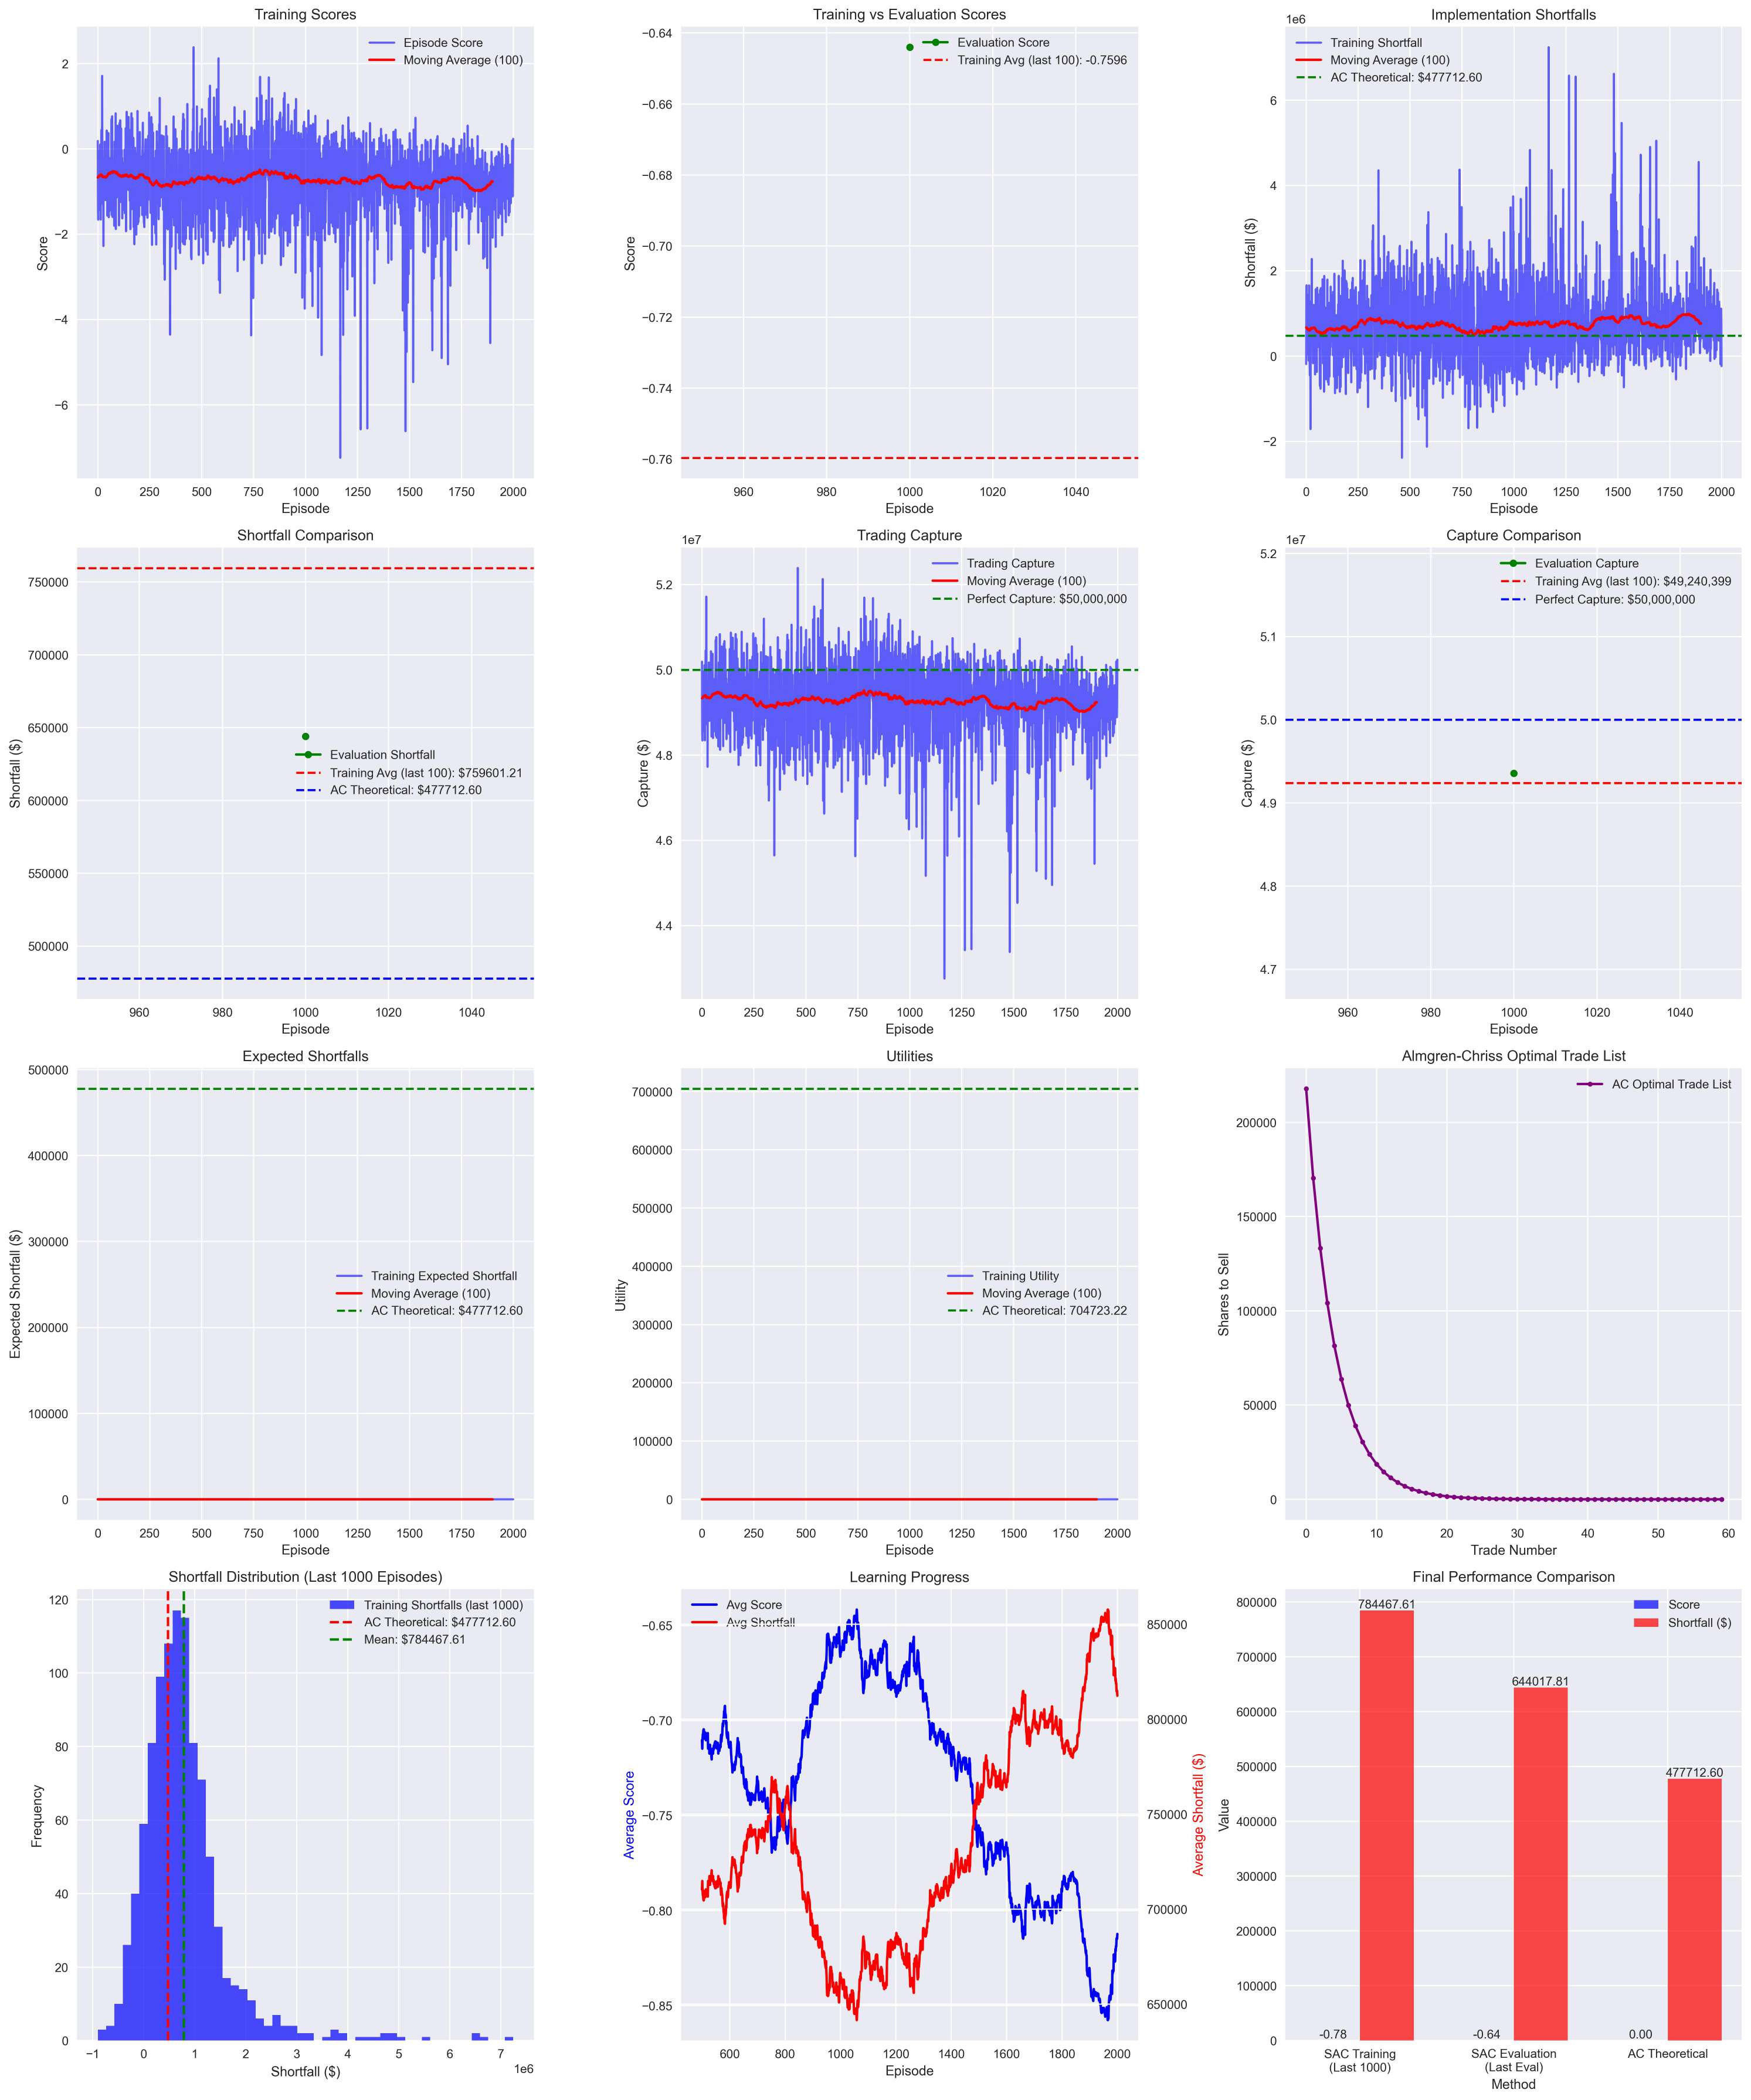
\includegraphics[width=0.4\linewidth]{sac_comprehensive_results.pdf}
		\caption{SAC training results}
	\end{figure}
\end{frame}

\begin{frame}{AC vs.\ DDPG vs.\ TD3 vs.\ SAC}
	\begin{itemize}
		\item \textbf{AC (Almgren–Chriss):}
		\begin{itemize}
			\item Analytically elegant baseline under ABM and linear impact.
			\item Inflexible in non-stationary or complex regimes.
		\end{itemize}
		
		\item \textbf{DDPG:}
		\begin{itemize}
			\item Learns adaptive, nonlinear execution policy.
			\item Strong performance in GBM/AR(L) scenarios.
			\item Training is sensitive to initialization and hyperparameters.
		\end{itemize}
		
		\item \textbf{TD3:}
		\begin{itemize}
			\item Fixes overestimation bias in DDPG.
			\item More consistent and stable learning.
		\end{itemize}
		
		\item \textbf{SAC:}
		\begin{itemize}
			\item Stochastic policy improves robustness and tail-risk.
			\item Less sensitive to tuning, handles uncertainty better.
		\end{itemize}
	\end{itemize}
\end{frame}
\begin{frame}{Final Recommendation}
	\begin{itemize}
		\item \textbf{AC is useful as a benchmark}, especially for gaining intuition and computing quick baselines.
		\item \textbf{RL methods dominate in complex environments}: GBM, AR(L), or nonlinear objectives.
		\item \textbf{Best Performer:} SAC provided the most stable and robust execution with lowest tail-risk.
		\item \textbf{Close Second:} TD3 performed slightly better than DDPG, especially in terms of stability.
		\item \textbf{Deployment Suggestion:} Use AC as a sanity check; use SAC as the main model for real-time policy generation.
	\end{itemize}
\end{frame}
\begin{frame}[allowframebreaks]{References}
		\tiny
		\bibliographystyle{abbrv}
		\begin{thebibliography}{9}
			\bibitem{AC2001} R. Almgren and N. Chriss. \emph{Optimal Execution of Portfolio Transactions}. 2001.
			\bibitem{Gatheral2012} J. Gatheral and A. Schied. \emph{Optimal Trade Execution under GBM}. 2012.
			\bibitem{Cheridito2025} P. Cheridito and M. Weiss. \emph{Reinforcement Learning for Trade Execution with Market Impact}. arXiv:2507.06345, 2025.
			\bibitem{Hafsi2024} Y. Hafsi and E. Vittori. \emph{Optimal Execution with Reinforcement Learning}. arXiv:2411.06389, 2024.
		\end{thebibliography}
\end{frame}
\end{document}